\documentclass[a4paper,12pt,twoside]{article}
\usepackage[left=1in,right=1in,top=1in,bottom=1in]{geometry}

\usepackage{xeCJK}
\setCJKmainfont{Songti TC}
\setCJKfamilyfont{kai}{Songti TC}
\newcommand{\kai}{\CJKfamily{kai}} % 用 \kai{使用楷書}

\usepackage{lmodern}
\usepackage{titling}
\usepackage{titlesec}
\usepackage{graphicx}
\usepackage{float}
\usepackage{amsmath, amsthm, amssymb, amsfonts, mathrsfs}
\usepackage{upgreek} % 直立的希臘字母

\usepackage[shortlabels]{enumitem}
\usepackage{setspace}
\renewcommand{\baselinestretch}{1.5}
\usepackage[colorlinks]{hyperref}
\usepackage{fancyvrb}
\usepackage{fancyhdr}
\usepackage{multicol}
\usepackage{caption}
\usepackage{listings}
\usepackage{bm}
\usepackage{bbm} % for \mathbbm{1} (indicator function)
\usepackage{centernot}
\usepackage{mdframed}
\usepackage{tikz}
\usetikzlibrary{patterns, arrows.meta, positioning}
\usepackage[nameinlink, capitalise]{cleveref}
\usepackage{diagbox}
\usepackage{booktabs}
\usepackage{multirow,array}
\usepackage{tabularx}
\usepackage{mathtools}
\usepackage{indentfirst} % 首段 indent
\setlength{\parindent}{2em}
\usepackage{cancel} % 數學式子畫線槓掉
\newcommand\mcancel[2][red]{\setbox0=\hbox{$#2$}%
\rlap{\raisebox{.45\ht0}{\textcolor{#1}{\rule{\wd0}{1pt}}}}#2}
\usepackage{datetime2}

\AtBeginDocument{%
 \setlength{\abovedisplayskip}{6pt}
 \setlength{\belowdisplayskip}{6pt}
 \setlength{\abovedisplayshortskip}{4pt}
 \setlength{\belowdisplayshortskip}{4pt}
}

\definecolor{codegreen}{rgb}{0,0.6,0}
\definecolor{codegray}{rgb}{0.5,0.5,0.5}
\definecolor{codepurple}{rgb}{0.58,0,0.82}
\definecolor{backcolour}{rgb}{0.95,0.95,0.92}

\lstdefinestyle{mystyle}{
 backgroundcolor=\color{backcolour},
 commentstyle=\color{codegreen},
 keywordstyle=\color{magenta},
 numberstyle=\tiny\color{codegray},
 stringstyle=\color{codepurple},
 basicstyle=\ttfamily\footnotesize,
 breakatwhitespace=false,
 breaklines=true,
 captionpos=b,
 keepspaces=true,
 numbers=left,
 numbersep=5pt,
 showspaces=false,
 showstringspaces=false,
 showtabs=false,
 tabsize=2
}
\lstset{style=mystyle}

\hypersetup{citecolor=blue, linkcolor=blue, urlcolor=blue}

\DeclareMathOperator{\supp}{supp}
\DeclareMathOperator{\skewness}{Skewness}
\DeclareMathOperator{\DU}{D-U}
\DeclareMathOperator{\CU}{C-U}
\DeclareMathOperator{\Geo}{Geo}
\DeclareMathOperator{\Pois}{Pois}
\DeclareMathOperator{\Gam}{Gam}
\DeclareMathOperator{\LN}{LogN}
\DeclareMathOperator{\cov}{Cov}
\DeclareMathOperator*{\argmax}{arg\,max}
\DeclareMathOperator*{\argmin}{arg\,min}
\DeclareMathOperator{\re}{Re}
\DeclareMathOperator{\im}{Im}

\newcommand{\N}{\mathbb{N}}
\newcommand{\Z}{\mathbb{Z}}
\newcommand{\Q}{\mathbb{Q}}
\newcommand{\R}{\mathbb{R}}
\newcommand{\C}{\mathbb{C}}
\newcommand{\G}{\mathcal{G}}
\newcommand{\mP}{\mathbb{P}}
\newcommand{\F}{\mathcal{F}}
\newcommand{\B}{\mathcal{B}}
\newcommand{\1}{\mathbbm{1}}
\newcommand{\Poi}{\text{Poi}}
\newcommand{\Var}{\text{Var}}
\newcommand{\as}{\text{a.s.}}
\newcommand{\vect}[1]{\boldsymbol{\mathbf{#1}}}
\newcommand{\paren}[1]{\left({#1}\right)}
\newcommand{\brk}[1]{\left[{#1}\right]}
\newcommand{\curl}[1]{\left\{{#1}\right\}}
\renewcommand{\lambda}{\lambdaup}

\theoremstyle{definition} % 定理環境 style 改用正體
\newtheorem{theorem}{定理}
\newtheorem{definition}{定義}
\newtheorem*{definition*}{定義}
\newtheorem{example}{例子}
\newtheorem{exercise}{練習}
\newtheorem{corollary}{推論}
\newtheorem{property}{性質}
\newtheorem{prop}{命題}
\newtheorem{lemma}{引理}
\newtheorem{problem}{問題}
\newtheorem*{remark}{註}

\renewcommand{\figurename}{圖}
\renewcommand{\tablename}{表}

\DeclareMathOperator{\var}{Var}
\DeclareMathOperator{\corr}{corr}
\DeclareMathOperator{\rank}{rank}
\DeclareMathOperator{\MSE}{MSE}
\DeclareMathOperator{\SSE}{SSE}
\DeclareMathOperator{\SST}{SST}
\DeclareMathOperator{\SSR}{SSR}
\DeclareMathOperator{\sgn}{sign}
\DeclareMathOperator{\alt}{Alt}
\DeclareMathOperator{\adj}{adj}
\DeclareMathOperator{\curlOp}{curl}
\DeclareMathOperator{\spn}{span}
\DeclareMathOperator{\sse}{SSE}
\DeclareMathOperator{\tr}{tr}

\newcommand{\ep}{\varepsilon}
\newcommand{\p}{\partial}
\newcommand{\abs}[1]{\left|#1\right|}
\newcommand\norm[1]{\left\lVert#1\right\rVert}
\newcommand{\innerprod}[1]{\langle#1\rangle}
\newcommand{\ds}{\displaystyle}
\newcommand{\blank}{\rule[-1mm]{1.5cm}{0.1mm}}
\newcommand{\dint}{\displaystyle\int}
\renewcommand{\bar}{\overline}

\newtheoremstyle{remark}{}{}{}{}{\bfseries\sffamily}{.}{.5em}{#1}
\theoremstyle{remark}

\newtheorem*{remark*}{\textit{Remark}}
\newtheorem*{solution*}{解}

\AtEndEnvironment{solution*}{\hfill$\square$}
\newtheorem*{hint*}{Hint}


\newcommand{\redtext}[1]{{\color{red} #1}}
\newcommand{\bluetext}[1]{{\color{blue} #1}}
\newenvironment{example-non}[1][]{\vspace{0.8em}\noindent\textbf{#1}\quad}{\vspace{0.8em}}
\newenvironment{solution}{\par\noindent\textbf{解}\quad}{\par\vspace{0.8em}}

\usepackage{xltabular}
\usepackage{tcolorbox}
\tcbuselibrary{skins,breakable}
\usetikzlibrary{patterns,decorations.pathreplacing,decorations.markings,decorations.shapes,decorations.pathmorphing,calc,3d}

\fancypagestyle{firstpage}{
  \fancyhf{}
  \fancyhead[R]{\small《高中數學實驗教材》第 5 冊（自然組）}
  \fancyhead[L]{\small 第 2 章\quad 排列組合}
  \fancyfoot[C]{\thepage}
}

\pagestyle{fancy}
\setlength{\headheight}{14pt}
\renewcommand{\headrulewidth}{0.5pt}
\renewcommand{\footrulewidth}{0pt}
\fancyhead{}
\fancyhead[LE]{\small 《高中數學實驗教材》第五冊（自然組）}
\fancyhead[RO]{\small 第二章\quad 排列組合}
\fancyfoot[C]{\thepage}

\title{\LARGE\textbf{《高中數學實驗教材》第五冊（自然組）}\\[0.5em] \Large\textbf{第二章\quad 排列組合}}
\author{\textbf{高中數學實驗教材編輯小組}\quad 編著}
\date{民國六十四年（1975）再版}

\begin{document}

\maketitle
\thispagestyle{firstpage}

% ==========================================
% 掃描檔勘誤、文字校訂與疑難處說明（依規則整理於目錄之前）
% ==========================================
\section*{【說明】第二章掃描檔勘誤、疑難處與文義校訂表}
\addcontentsline{toc}{section}{【說明】第二章掃描檔勘誤、疑難處與文義校訂表}
\label{sec:errata_notes_b5_ch2}

本章依據 1975 年再版《高中數學實驗教材 第五冊（自然組）》（高三上）第二章「排列組合」掃描原件完整轉錄為 \LaTeX{} 格式。為忠實反映教材原始內容並兼顧排版品質與嚴謹性，依作業規範將掃描檔中出現之印刷訛誤、符號缺漏、字模損毀、歷史印記雜訊及文義疑難處詳細考證彙整於下表。讀者可點擊表格中之章節連結直接跳至正文對應位置：

\small
\renewcommand{\arraystretch}{1.35}
\begin{xltabular}{\textwidth}{|p{3.2cm}|p{3.8cm}|X|}
\caption{第二章掃描檔勘誤、疑難處與文義校訂表}\label{tab:errata_b5_ch2} \\
\hline
\textbf{章節位置} & \textbf{掃描檔原始現象 / 誤植} & \textbf{考證說明與校訂處理} \\ \hline
\endfirsthead
\hline
\textbf{章節位置} & \textbf{掃描檔原始現象 / 誤植} & \textbf{考證說明與校訂處理} \\ \hline
\endhead
\hline
\endfoot

\hyperref[note:b5-ch2-p58-k]{§ II-1 頁 58 基本計數原則} & 
「如果 $A_1, A_2, \cdots, A_k$ 是個有限集合」 & 
原書漏印集合個數「$k$」，脫漏作「是個有限集合」，茲據文義校補為「是 $k$ 個有限集合」． \\ \hline

\hyperref[note:b5-ch2-p60-a3]{§ II-1 頁 60 路線走法說明} & 
「由 $A_0$ 經 $A_1, A_2$ 到 $A^3$ 共有 105 種走法」 & 
原書節點誤植為上標「$A^3$」，茲據文意與圖 2-1 標記校正為下標「$A_3$」． \\ \hline

\hyperref[note:b5-ch2-linear-perm]{§ II-2 頁 69 乙段標題} & 
「乙、線形排列」 & 
原書標題及內文作「線形排列」，即現行通稱之「直線排列」或「線性排列」，保留原文並加註說明． \\ \hline

\hyperref[note:b5-ch2-p72-go-stones]{§ II-2 頁 72 論例 7(ii)} & 
「白子 5 個，黑子 5 點」 & 
原書作「5 點」，即「5 個（顆）」之意，保留原文並加註說明． \\ \hline

\hyperref[note:b5-ch2-p72-surjection-period]{§ II-2 頁 72 論例 7(ii)} & 
「則映射到黑子，白子各 5 次的蓋射個數。」 & 
解答句末贅印句號，予以註記說明． \\ \hline

\hyperref[note:b5-ch2-p74-ex14]{§ II-2 頁 74 土風舞引述} & 
「例如在例 14 (ii) 中跳土風舞時」 & 
實為第 70 頁之〔例 11〕(ii)，此處係原書例題編號錯參，特加註校訂． \\ \hline

\hyperref[note:b5-ch2-p75-q6-quote]{§ II-2 頁 75 習題 II-2 第 6 題} & 
「某社區巷道如右圖，‘早晨派報時」 & 
「如右圖」後贅印單引號「‘」，正文予以刪除並加註說明． \\ \hline

\hyperref[note:b5-ch2-p75-q7-crayon]{§ II-2 頁 75 習題 II-2 第 7 題} & 
「小明有 12 色臘筆」 & 
「臘」通「蠟」，即蠟筆，保留原文並加註說明． \\ \hline

\hyperref[note:b5-ch2-p75-eq]{§ II-3 頁 75 定理 7 釋例} & 
「例如 $C_2^5 == \frac{5!}{(5-2)! 2!}$」 & 
原書多印一個等號「$==$」，茲更正為單個等號「$=$」． \\ \hline

\hyperref[note:b5-ch2-p76-east6]{§ II-3 頁 76 走法組合分析} & 
「向東段及向北 3 段」 & 
原書漏印數字「6」，依上下文「共走九小段」校補為「向東 6 段及向北 3 段」． \\ \hline

\hyperref[note:b5-ch2-p76-thm8-dots]{§ II-3 頁 76 定理 8} & 
「$|B| = n$，\dots 及 $C = \{0, 1\}$」 & 
此處省略號「\dots」為原書原文，疑為承接前段排版遺留，保留原文並加註說明． \\ \hline

\hyperref[note:b5-ch2-p77-cb]{§ II-3 頁 77 映射個數} & 
「$|C^B| = |C^n| = 2^n \mid$」 & 
原書符號印刷雜訊，末尾豎線疑為雜點，且集合之勢實為 $|C|^n$，加註說明． \\ \hline

\hyperref[note:b5-ch2-p77-pn]{§ II-3 頁 77 冪集式 (3)} & 
「$|\mathscr{P}(B)| = |C^n| = 2^n$」 & 
原書若將映射集合視為笛卡兒積 $C^n$，其勢記為 $|C^n|$，即 $|C|^n = 2^n$，加註說明． \\ \hline

\hyperref[note:b5-ch2-p83-zhankai]{§ II-3 頁 83 論例 10} & 
「如將 $(x_1 + \dots + x_n)^m$ 展開式 $m$ 次齊次式」 & 
原書作「展開式」，依文意校正為「展開成 $m$ 次齊次式」． \\ \hline

\hyperref[note:b5-ch2-p83-gongyong]{§ II-3 頁 83 習題 II-3 第 2 題} & 
「共用幾種可能派法？」 & 
原書作「共用」，疑為「共有」之誤植，保留原文並加註說明． \\ \hline

\hyperref[note:b5-ch2-p85-expand]{§ II-4 頁 85 展開項次序} & 
「$xx\cdots xx + xx\cdots xy + xx\cdots xyx + \cdots$」 & 
照原書字典順序展開排印並加註說明省略項次序． \\ \hline

\hyperref[note:b5-ch2-p90-binom]{§ II-4 頁 90 式 (4) 展開} & 
雙重求和內原印作「$\binom{n}{k} \binom{k}{j}$」 & 
其中「$\binom{n}{k}$」顯係「$\binom{m}{k}$」之印刷訛誤，茲更正為 $\binom{m}{k}$． \\ \hline

\hyperref[note:b5-ch2-p90-ex11-typo]{§ II-4 頁 90 論例 11} & 
「將 $(x+y+y)^4$ 展開」 & 
原書誤植第二個 $y$，顯係「$(x+y+z)^4$」之訛誤，更正為 $(x+y+z)^4$． \\ \hline

\hyperref[note:b5-ch2-p90-ex11-y4]{§ II-4 頁 90 論例 11 解答} & 
括弧內印作「$(x^4 + x^4 + z^4)$」 & 
第二項「$x^4$」顯係「$y^4$」之誤，茲更正為 $x^4 + y^4 + z^4$． \\ \hline

\hyperref[note:b5-ch2-p90-disc10]{§ II-4 頁 90 論例 11 說明} & 
「由論例 10 知上式有 $H_4^3 = 15$ 個不同類項」 & 
加註指明引用前節（§ II-3 重複組合）之論例 10． \\ \hline

\hyperref[note:b5-ch2-p91-eq5]{§ II-4 頁 91 定理 11} & 
定理 11 右端漏印公式標號 & 
後文推導明確稱「如在 (5) 中令 $x_1 = \cdots = x_n = 1$」，依文意補上編號 (5)． \\ \hline

\hyperref[note:b5-ch2-p91-p1]{§ II-4 頁 91 定理 11 證明} & 
「故應用 $P!$ 去除」 & 
漏印足標 1，依文義校訂為「$P_1!$」． \\ \hline

\hyperref[note:b5-ch2-p91-pm]{§ II-4 頁 91 定理 11 證明} & 
分母末項印作「$P_m!$」 & 
依變數個數 $n$ 應為「$P_n!$」，更正為 $P_n!$． \\ \hline

\hyperref[note:b5-ch2-p91-right]{§ II-4 頁 91 定理 11 說明} & 
「左邊為...重複排列總數，左邊的各項則為...」 & 
第二個「左邊」顯為「右邊」之筆誤，茲更正為「右邊」． \\ \hline

\hyperref[note:b5-ch2-p92-q3-3]{§ II-4 頁 92 習題 II-4 第 3(3) 題} & 
「$\left(2x^2 + \frac{3}{x}\right)^5$ 中 $x^3$ 的係數」 & 
展開式各項指數為 $10-3k \ne 3$，不存在 $x^3$ 項（係數為 0），保留原文並加註說明． \\ \hline

\end{xltabular}

\vspace{1em}
\hrule
\vspace{1em}

\tableofcontents
\newpage

% ==============================================================================
% 第二章 排列組合
% ==============================================================================
\section{排列組合}\label{sec:b5-ch2}

\begin{center}
\begin{minipage}{0.75\textwidth}
\begin{itemize}[leftmargin=2em, itemsep=0.3em]
  \item[§ II-1] \textbf{有限集合}
  \begin{itemize}[leftmargin=2em, itemsep=0.2em]
    \item[甲、] 直\quad 積
    \item[乙、] 映\quad 射
  \end{itemize}
  \item[§ II-2] \textbf{排\quad 列}
  \begin{itemize}[leftmargin=2em, itemsep=0.2em]
    \item[甲、] 重複排列
    \item[乙、] 線性排列
    \item[丙、] 環狀排列
  \end{itemize}
  \item[§ II-3] \textbf{組\quad 合}
  \begin{itemize}[leftmargin=2em, itemsep=0.2em]
    \item[甲、] 組\quad 合
    \item[乙、] 重複組合
  \end{itemize}
  \item[§ II-4] \textbf{二項式定理}
  \begin{itemize}[leftmargin=2em, itemsep=0.2em]
    \item[甲、] 二項式定理
    \item[乙、] 多項式定理
  \end{itemize}
\end{itemize}
\end{minipage}
\end{center}

\begin{center}
$* \qquad * \qquad * \qquad * \qquad *$
\end{center}

在本章中我們介紹排列與組合的基本概念，一般規則，以及若干有系統的計數方法，雖然，排列與組合只是有限集合的理論，但是它的應用範圍都非常廣泛，這是因為不論在日常生活或科學研究方面，很多實際問題所涉及的事物都是有限的，都可以作為有限集合來討論，在下一章要講的機率就是排列與組合的一項重要應用，許多機率問題都要利用排列與組合的方法來計算．

% ==============================================================================
% § II-1 有限集合
% ==============================================================================
\subsection{有限集合}\label{sec:b5-2-1}

因為排列與組合所討論的是有關有限集合的問題，所以我們要對有限集合有較為深入的了解，在這一節中我們首先引入集合的直積，複習映射的性質，再進一步討論有限集合到有限集合的映射．

\subsubsection*{甲、直積}

\noindent\textbf{定義}\quad 設 $A, B$ 是兩個任意（有限的或無限的）集合，則所有元素序對 $(x, y)$，$x \in A, y \in B$，所成的集合稱為 $A$ 與 $B$ 的直積，記做 $A \times B$，也就是說
\[
A \times B = \{(x, y) \mid x \in A, y \in B\}
\]
一般地，設 $A_1, A_2, \ldots, A_n$ 是 $n$ 個任意集合，則所有元素序組 $(x_1, x_2, \ldots, x_n)$，$x_i \in A_i,\; i = 1, \ldots, n$，所成的集合稱為 $A_1, A_2, \ldots, A_n$ 的直積，記做 $A_1 \times A_2 \times \cdots \times A_n$，也就是說
\[
A_1 \times A_2 \times \cdots \times A_n = \{(x_1, x_2, \ldots, x_n) \mid x_i \in A_i,\; i = 1, \ldots, n\}
\]
由定義可知，當 $A \ne B$ 時，$A \times B \ne B \times A$，當 $B = A$ 時，$A$ 與 $B$ 的直積卽成為 $A$ 與 $A$ 本身的直積，這時我們把它簡記為 $A^2$，亦卽
\begin{align*}
A^2 = A \times A &= \{(x, y) \mid x \in A, y \in A\} \\
&= \{(x, y) \mid x, y \in A\}
\end{align*}
由此類推，$n$ 個相同集合 $A$ 的直積則簡記為 $A^n$，亦卽
\[
A^n = \underbrace{A \times \cdots \times A}_{n\text{ 個}} = \{(x_1, \ldots, x_n) \mid x_i \in A,\; i = 1, \ldots, n\}
\]

\medskip
\noindent\textbf{〔例 1〕} 實數集合 $\mathbf{R}$ 與 $\mathbf{R}$ 本身的直積
\[
\mathbf{R}^2 = \mathbf{R} \times \mathbf{R} = \{(x, y) \mid x \in \mathbf{R}, y \in \mathbf{R}\}
\]
當我們考慮實數集合 $\mathbf{R}$ 與實數直線的一一對應時，則 $\mathbf{R}^2$ 卽與 $x\,y$ 平面一一對應．

同理 $\mathbf{R}^3 = \mathbf{R} \times \mathbf{R} \times \mathbf{R}$ 則與 $x\,y\,z$-空間一一對應．\hfill $\#$

\medskip
\noindent\textbf{〔例 2〕} 設有限集合 $A=\{a_1, a_2, a_3\}$，$B=\{b_1, b_2\}$，則 $A$ 與 $B$ 的直積，
\[
A \times B = \{(a_1, b_2), (a_1, b_1), (a_2, b_1), (a_2, b_2), (a_3, b_1), (a_3, b_2)\}
\]
而 $B$ 與 $A$ 的直積為
\[
B \times A = \{(b_1, a_1), (b_1, a_2), (b_1, a_3), (b_2, a_1), (b_2, a_2), (b_2, a_3)\}
\]
顯然 $A \times B \ne B \times A$．

直積 $A \times B$ 中的元素可以依照平面上點以座標方法表示（見下面左圖），也可以用列表方式表示（下面右圖）：

\begin{figure}[H]
\centering
\begin{minipage}[c]{0.45\textwidth}
\centering
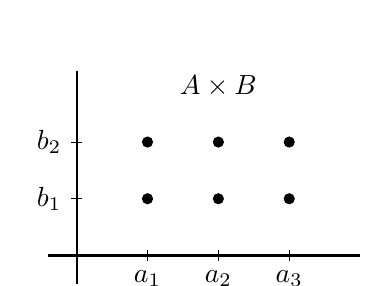
\begin{tikzpicture}[scale=0.9, >=Stealth]
  % Axes
  \draw[thick] (-0.4, 0) -- (4.0, 0);
  \draw[thick] (0, -0.4) -- (0, 2.6);
  \node[above] at (2.0, 2.1) {$A \times B$};
  
  % Ticks on x-axis
  \draw (1.0, 0.08) -- (1.0, -0.08) node[below] {$a_1$};
  \draw (2.0, 0.08) -- (2.0, -0.08) node[below] {$a_2$};
  \draw (3.0, 0.08) -- (3.0, -0.08) node[below] {$a_3$};
  
  % Ticks on y-axis
  \draw (0.08, 0.8) -- (-0.08, 0.8) node[left] {$b_1$};
  \draw (0.08, 1.6) -- (-0.08, 1.6) node[left] {$b_2$};
  
  % Points
  \foreach \x in {1.0, 2.0, 3.0} {
    \foreach \y in {0.8, 1.6} {
      \filldraw (\x, \y) circle (2pt);
    }
  }
\end{tikzpicture}
\end{minipage}
\qquad
\begin{minipage}[c]{0.45\textwidth}
\centering
\renewcommand{\arraystretch}{1.3}
\begin{tabular}{c|cc}
\diagbox[width=1.8cm, height=0.9cm]{$A$}{$B$} & $b_1$ & $b_2$ \\ \hline
$a_1$ & $(a_1, b_1)$ & $(a_1, b_2)$ \\
$a_2$ & $(a_2, b_1)$ & $(a_2, b_2)$ \\
$a_3$ & $(a_3, b_1)$ & $(a_3, b_2)$
\end{tabular}
\end{minipage}
\hfill $\#$
\end{figure}

現設 $A$ 為任意有限集合，我們用 $|A|$ 表示 $A$ 中所含元素個數，（在第一冊中曾用 $n(A)$ 表示，現在為避免混淆，改用 $|A|$），如果 $A$ 中共有 $m$ 個元素，則 $|A| = m$，對於直積中所含元素個數，我們有下列基本計數原則：

\medskip
\noindent\textbf{【基本計數原則】}如果 $A, B$ 是兩個有限集合，則
\begin{equation}
|A \times B| = |A| \cdot |B| \tag{1}
\end{equation}
更進一步，如果 $A_1, A_2, \ldots, A_k$ 是 $k$ 個有限集合\phantomsection\label{note:b5-ch2-p58-k}\footnote{【原書註記/校訂】：原書此處脫漏「$k$」字，作「是個有限集合」，茲據文義校補為「是 $k$ 個有限集合」．}，則
\begin{equation}
|A_1 \times A_2 \times \cdots \times A_k| = |A_1| \cdot |A_2| \cdots\cdots |A_k| \tag{2}
\end{equation}
也就是說，直積中元素個數等於各集合中元素個數的乘積．

\medskip
\noindent\textbf{證明：}設 $A = \{a_1, a_2, \ldots, a_m\}$，$B = \{b_1, \ldots, b_n\}$，則
\[
A \times B = \{(a_i, b_j) \mid i = 1, \ldots, m,\; j = 1, \ldots, n\}
\]
取定 $i = 1$ 時，我們可自 $A \times B$ 中選出 $n$ 個元素
\[
(a_1, b_1), (a_1, b_2), \ldots, (a_1, b_n)
\]
同理當 $i = 2, \ldots, m$ 時，也各自得到 $n$ 個元素，將 $i$ 自 $1$ 至 $m$ 累計，卽得到總數 $m \cdot n$ 個元素，亦卽
\[
|A \times B| = |A| \cdot |B| = m \times n
\]
對於 $A_1 \times A_2 \times \cdots \times A_k$ 的情形，我們可以利用數學歸納法來證明．$k = 2$ 的情形上面已經證明成立，假設 $k - 1$ 時主張成立，卽設
\begin{equation}
|A_1 \times A_2 \times \cdots \times A_{k-1}| = |A_1| \cdot |A_2| \cdots\cdots |A_{k-1}| \tag{3}
\end{equation}
現在考慮直積 $A_1 \times A_2 \times \cdots \times A_k$，我們先要證明
\begin{equation}
|A_1 \times \cdots \times A_{k-1} \times A_k| = |(A_1 \times \cdots \times A_{k-1}) \times A_k| \tag{4}
\end{equation}
式中 $(A_1 \times \cdots \times A_{k-1}) \times A_k$ 表示集合 $A_1 \times \cdots \times A_{k-1}$ 與 $A_k$ 的直積，對於 $x_i \in A_i,\; i = 1, \ldots, k$，我們定義下列對應
\[
(x_1, \ldots, x_{k-1}, x_k) \longleftrightarrow ((x_1, \ldots, x_{k-1}), x_k)
\]
這個對應顯然為 $A_1 \times \cdots \times A_{k-1} \times A_k$ 與 $(A_1 \times \cdots \times A_{k-1}) \times A_k$ 之間的一一對應，由此可知這兩個集合中元素個數相等，亦卽 (4) 式成立，對於 $A_1 \times \cdots \times A_{k-1}$ 與 $A_k$ 兩個集合的直積，我們有
\[
|(A_1 \times \cdots \times A_{k-1}) \times A_k| = |A_1 \times \cdots \times A_{k-1}| \cdot |A_k|
\]
將 (3) 式代入上式右邊卽得所要證明的 (2) 式．\hfill $\#$

\medskip
基本計數原則也可以寫成下列方便實用的形式：

如果做一件事有 $k$ 個步驟，而第 $j$ 個步驟，可以用 $m_j$ 個方法去做，$(j = 1, \ldots, k)$，則做這件事就有
\[
m_1 m_2 \cdots m_k
\]
種方法．

例如在下面的路線圖中，由 $A_0$ 到 $A_1$ 有 3 種走法，由 $A_1$ 到 $A_2$ 有 5 種走法，由 $A_2$ 到 $A_3$ 有 7 種走法．因此由 $A_0$ 經 $A_1, A_2$ 到 $A_3$\phantomsection\label{note:b5-ch2-p60-a3}\footnote{【原書註記/校訂】：原書此處誤植為上標「$A^3$」，茲據文義與圖 2-1 校訂為下標「$A_3$」．}共有 $3 \cdot 5 \cdot 7 = 105$ 種走法．

\begin{figure}[H]
\centering
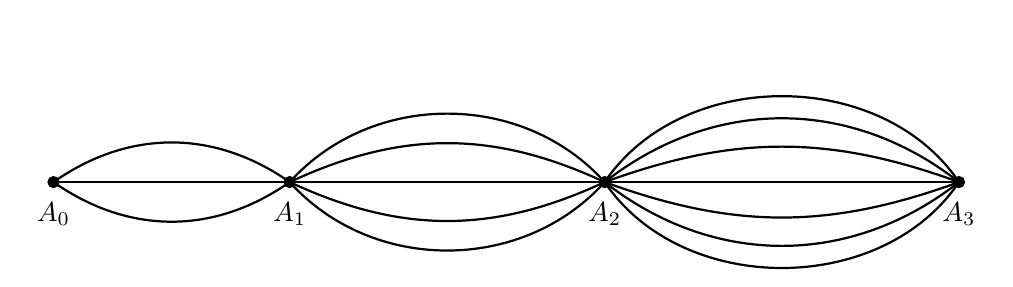
\begin{tikzpicture}[scale=1.0, >=Stealth]
  \coordinate (A0) at (0, 0);
  \coordinate (A1) at (3.0, 0);
  \coordinate (A2) at (7.0, 0);
  \coordinate (A3) at (11.5, 0);

  % Between A0 and A1: 3 paths
  \draw[thick] (A0) -- (A1);
  \draw[thick] (A0) to[out=35, in=145] (A1);
  \draw[thick] (A0) to[out=-35, in=-145] (A1);

  % Between A1 and A2: 5 paths
  \draw[thick] (A1) -- (A2);
  \draw[thick] (A1) to[out=25, in=155] (A2);
  \draw[thick] (A1) to[out=48, in=132] (A2);
  \draw[thick] (A1) to[out=-25, in=-155] (A2);
  \draw[thick] (A1) to[out=-48, in=-132] (A2);

  % Between A2 and A3: 7 paths
  \draw[thick] (A2) -- (A3);
  \draw[thick] (A2) to[out=20, in=160] (A3);
  \draw[thick] (A2) to[out=38, in=142] (A3);
  \draw[thick] (A2) to[out=56, in=124] (A3);
  \draw[thick] (A2) to[out=-20, in=-160] (A3);
  \draw[thick] (A2) to[out=-38, in=-142] (A3);
  \draw[thick] (A2) to[out=-56, in=-124] (A3);

  % Nodes
  \filldraw (A0) circle (2pt) node[below=4pt] {$A_0$};
  \filldraw (A1) circle (2pt) node[below=4pt] {$A_1$};
  \filldraw (A2) circle (2pt) node[below=4pt] {$A_2$};
  \filldraw (A3) circle (2pt) node[below=4pt] {$A_3$};
\end{tikzpicture}
\caption*{圖 2-1}
\label{fig:b5-2-1}
\end{figure}

設有限集合 $A$ 的元素個數 $|A| = m$，考慮 $k$ 個 $A$ 的直積，由上述計數原則卽得
\begin{equation}
|A^k| = |\underbrace{A \times \cdots \times A}_{k\text{ 個}}| = \underbrace{|A| \cdots\cdots |A|}_{k\text{ 個}} = |A|^k = m^k \tag{5}
\end{equation}
當 $k = 2$ 時，我們把 $A^2$ 的子集
\[
D = \{(x, x) \mid x \in A\} \subset A^2
\]
稱為 $A^2$ 的對角線，顯然
\[
|D| = |A| = m
\]

\begin{figure}[H]
\centering
\begin{tikzpicture}[scale=1.0, >=Stealth]
  % Axes
  \draw[thick] (-0.3, 0) -- (4.8, 0) node[right=2pt] {$A$};
  \draw[thick] (0, -0.3) -- (0, 4.8) node[above=2pt] {$A$};

  % Ticks on x-axis
  \draw (0.8, 0.08) -- (0.8, -0.08) node[below=2pt] {$a_1$};
  \draw (1.6, 0.08) -- (1.6, -0.08) node[below=2pt] {$a_2$};
  \draw (3.8, 0.08) -- (3.8, -0.08) node[below=2pt] {$a_m$};

  % Ticks on y-axis
  \draw (0.08, 0.8) -- (-0.08, 0.8) node[left=2pt] {$a_1$};
  \draw (0.08, 1.6) -- (-0.08, 1.6) node[left=2pt] {$a_2$};
  \draw (0.08, 3.8) -- (-0.08, 3.8) node[left=2pt] {$a_m$};

  % Dashed lines
  % Diagonal
  \draw[thick, dashed] (0.3, 0.3) -- (4.3, 4.3);

  % Vertical dashed lines
  \draw[thick, dashed] (0.8, 0.8) -- (0.8, 3.8);
  \draw[thick, dashed] (1.6, 1.6) -- (1.6, 3.8);
  \draw[thick, dashed] (3.8, 0) -- (3.8, 3.8);

  % Horizontal dashed line
  \draw[thick, dashed] (0, 3.8) -- (3.8, 3.8);

  % Points
  \filldraw (0.8, 0.8) circle (2pt);
  \filldraw (1.6, 1.6) circle (2pt);
  \filldraw (3.8, 3.8) circle (2pt);
  \filldraw (0.8, 3.8) circle (2pt);
  \filldraw (1.6, 3.8) circle (2pt);
\end{tikzpicture}
\end{figure}

因此差集
\begin{equation}
|A^2 - D| = m^2 - m = m(m-1) \tag{6}
\end{equation}
也就是說 $A^2$ 中前後成分不相等的元素 $(x, y)$，$x \ne y$ 的個數等於 $m(m-1)$．

在一般情形，我們有下列定理：

\medskip
\noindent\textbf{【定理 1】}設有限集合 $A$ 中元素個數 $|A| = m$，令 $E$ 表示 $A^k$ ($1 \le k \le m$) 中各成分互不相等的元素所成的子集，亦卽
\[
E = \{(x_1, \ldots, x_k) \mid x_1, \ldots, x_k \in A \text{ 但當 } i \ne j \text{ 時，} x_i \ne x_j\}
\]
則
\begin{equation}
|E| = \frac{m!}{(m-k)!} \tag{7}
\end{equation}
式中 $m! = m(m-1)\cdots\cdots 3 \cdot 2 \cdot 1$，$(m-k)! = (m-k)\cdots\cdots 3 \cdot 2 \cdot 1$（$m!$ 表示 $m, m-1, \ldots, 3, 2, 1$ 的連乘積，叫做 $m$ 的階乘，我們規定 $0$ 的階乘為 $0! = 1$）．

\medskip
\noindent\textbf{證明}\quad 我們對於 $k$ 用數學歸納法來證明．

對於 $k = 2$ 及任意 $m \ge 2$，則 $E$ 卽等於上一段中的 $A^2 - D$，而 (6) 式為 (7) 式的特別情形：
\[
|E| = |A^2 - D| = m(m-1) = \frac{m!}{(m-2)!}
\]
假設 $k-1$ 及 $m-1$ ($m-1 \ge k-1$) 時定理成立，考慮 $k$ 及 $m$ ($m \ge k$) 的情形，設
\[
A = \{a_1, \ldots, a_m\}
\]
我們觀察 $E$ 中所有第一成分為 $a_1$ 的元素所成的集合
\[
\{(a_1, x_2, \ldots, x_k) \mid x_2, \ldots, x_k \in A,\; x_2, \ldots, x_k \text{ 皆不等於 } a_1 \text{ 且互異}\}
\]
顯然此集合中的元素個數與下列集合（令 $A' = A - \{a_1\}$）
\[
\{(x_2, \ldots, x_k) \mid x_2, \ldots, x_k \in A' \text{ 且 } x_2, \ldots, x_k \text{ 互異}\} \subset A'^{k-1}
\]
中元素個數相等，但已假設 $k-1$ 時 (7) 式成立，故後一集合中元素個數為
\[
\frac{(m-1)!}{[(m-1)-(k-1)]!} = \frac{(m-1)!}{(m-k)!}
\]
此亦為 $E$ 中第一成分為 $a_1$ 的元素個數，同理對於 $a_2, \ldots, a_m$ 各得相同個數，因此
\[
|E| = m \cdot \frac{(m-1)!}{(m-k)!} = \frac{m!}{(m-k)!} \hfill \#
\]

\medskip
\noindent\textbf{〔例 3〕} 設 $A=\{1,2,3,4,5,6,7,8,9,10\}$，並令 $E$ 表示 $A^3$ 中各成分互不相等的元素所成的子集．則
\[
|E| = \frac{10!}{(10-3)!} = \frac{10!}{7!} = 10 \cdot 9 \cdot 8 = 720
\]

\subsubsection*{乙、映射}

設 $A, B$ 為兩個任意非空集合，則映射
\[
f : A \longrightarrow B
\]
將每一元素 $a \in A$ 映射到一個確定的元素 $b = f(a) \in B$，如果對於任意 $a_1, a_2 \in A$，$a_1 \ne a_2$，恆有 $f(a_1) \ne f(a_2)$，我們稱 $f$ 為 $A$ 到 $B$ 的\textbf{嵌射}（injection，卽一對一的映射），如果 $f(A) = B$ 成立我們則稱 $f$ 為 $A$ 到 $B$ 的\textbf{蓋射}（surjection，卽 $f$ 將 $A$ 映成 $B$），如果 $f$ 為嵌射且蓋射（一對一映成），則稱 $f$ 為\textbf{對射}（bijection）．

設 $A = B = \mathbf{R}$（實數集合），則在第一、二冊中我們已知以下諸函數均為從 $A$ 到 $B$ 的映射，且
\begin{enumerate}[label=(\roman*), topsep=2pt, itemsep=2pt]
  \item $f : x \longmapsto x^2$ 為 $A$ 到 $B$ 的映射，旣不是嵌射也不是蓋射．
  \item $f : x \longmapsto 2^x$ 為 $A$ 到 $B$ 的嵌射，但非蓋射．
  \item $f : x \longmapsto x^3 - x$ 為 $A$ 到 $B$ 的蓋射，但非嵌射．
  \item $f : x \longmapsto x^3$ 為 $A$ 到 $B$ 的對射．
\end{enumerate}
又若 $A = \mathbf{R} \times \mathbf{R}$，\quad $B = \mathbf{R} \times \mathbf{R}$，則
\[
f(x_1, x_2) = (a x_1 + b x_2, c x_1 + d x_2)
\]
為 $A$ 到 $B$ 的映射稱為線性映射（第四冊第一章）．

$f$ 若為嵌射，必為對射，其充要條件為 $ad - bc \ne 0$．

\medskip
\noindent\textbf{〔例 4〕} 設 $A=\{a, b, c\}, B=\{0, 1\}$
\begin{enumerate}[label=(\roman*), topsep=2pt, itemsep=4pt]
  \item 定義映射 $f : A \longrightarrow B$
  \[
  f : a \longmapsto 0,\quad b \longmapsto 0,\quad c \longmapsto 1
  \]
  則 $f$ 為 $A$ 到 $B$ 的蓋射．
  \item 定義映射 $g : B \longrightarrow A$
  \[
  g : 0 \longmapsto a,\quad 1 \longmapsto b,
  \]
  則 $g$ 為 $B$ 到 $A$ 的嵌射．
  \item 定義映射 $h : A \longrightarrow A$；
  \[
  h : a \longmapsto b,\quad b \longmapsto c,\quad c \longmapsto a,
  \]
  則 $h$ 為 $A$ 到 $A$ 的對射．\hfill $\#$
\end{enumerate}

\medskip
\noindent\textbf{〔例 5〕} 若 $A, B$ 皆為有限集合，設 $|A| = m$，$|B| = n$ 則由嵌射、蓋射及對射的意義可知：
\[
\left(
\begin{aligned}
&\text{若 } f \text{ 為嵌射（一對一），則 } m \le n\text{．} \\
&\text{若 } f \text{ 為蓋射（映成），則 } m \ge n\text{．} \\
&\text{若 } f \text{ 為對射（一對一映成），則 } m = n\text{．}
\end{aligned}
\right.
\]
當 $m = n$ 時，若 $f$ 為嵌射或蓋射，則顯然 $f$ 必為對射．\hfill $\#$

\medskip
下面我們要計算 $A$ 到 $B$ 的一般映射的個數．令 $B^A$ 表示所有自 $A$ 到 $B$ 的映射所成的集合（簡稱為 $A$ 到 $B$ 的映射集合），卽
\[
B^A = \{f \mid f \text{ 為 } A \text{ 到 } B \text{ 的映射}\}
\]
設 $A$ 為有限集合，為簡便計，我們設 $A = \{1, 2, \ldots, m\}$．若 $f \in B^A$，則 $f(i) = x_i \in B$，$i = 1, \ldots, m$，而用 $x_i$ 作成之序組，$(x_1, \ldots, x_m) \in B^m$．如此將 $B^A$ 中每一個元素，（卽一個映射）對應到 $B^m$ 中一個確定的元素，而且 $B^A$ 中不同的元素（卽不同的映射）對應到 $B^m$ 中不同的元素．這就是說，由對應
\[
f \longmapsto (f(1), \ldots, f(m)) \in B^m,\quad f \in B^A
\]
可定義出 $B^A$ 到 $B^m$ 的一個嵌射，反之對於任一 $(x_1, \ldots, x_m) \in B^m$ 我們可以由定義
\[
f(i) = x_i,\quad i = 1, \ldots, m,
\]
得到一個 $A$ 到 $B$ 的映射 $f$，而 $f \longmapsto (x_1, \ldots, x_m)$．

這表示所說的對應同時也是 $B^A$ 到 $B^m$ 的蓋射，因此為 $B^A$ 到 $B^m$ 的對射，這樣每一個 $A$ 到 $B$ 的映射都可以用 $B^m$ 中的一個元素來代表，因此在本質上我們對此二者可以不必加以區分，可將 $B^m$ 就看做 $A$ 到 $B$ 的映射集合．

由以上的討論，我們直接得到下列定理：

\medskip
\noindent\textbf{【定理 2】}設 $A, B$ 為有限集合，$|A| = m$，$|B| = n$，令 $B^A$ 表示所有 $A$ 到 $B$ 的映射所成的集合，則
\begin{equation}
|B^A| = |B^m| = n^m. \tag{8}
\end{equation}

\medskip
\noindent\textbf{【論例 1】}設 $A=\{1, 2, 3\}, B=\{a, b\}$，則 $|B^A| = 2^3 = 8$，實際上我們有下列 8 個映射：

\begin{center}
\renewcommand{\arraystretch}{1.2}
\begin{tabular}{r@{\quad}l@{\quad}|@{\quad}l}
\multicolumn{2}{c|}{$B^A$} & \multicolumn{1}{c}{$B^3$} \\ \hline
$f_1 :$ & $1 \longrightarrow a,\; 2 \longrightarrow a,\; 3 \longrightarrow a,$ & $f_1 \longrightarrow (a, a, a)$ \\
$f_2 :$ & $1 \longrightarrow a,\; 2 \longrightarrow a,\; 3 \longrightarrow b,$ & $f_2 \longrightarrow (a, a, b)$ \\
$f_3 :$ & $1 \longrightarrow a,\; 2 \longrightarrow b,\; 3 \longrightarrow a,$ & $f_3 \longrightarrow (a, b, a)$ \\
$f_4 :$ & $1 \longrightarrow b,\; 2 \longrightarrow a,\; 3 \longrightarrow a,$ & $f_4 \longrightarrow (b, a, a)$ \\
$f_5 :$ & $1 \longrightarrow a,\; 2 \longrightarrow b,\; 3 \longrightarrow b,$ & $f_5 \longrightarrow (a, b, b)$ \\
$f_6 :$ & $1 \longrightarrow b,\; 2 \longrightarrow a,\; 3 \longrightarrow b,$ & $f_6 \longrightarrow (b, a, b)$ \\
$f_7 :$ & $1 \longrightarrow b,\; 2 \longrightarrow b,\; 3 \longrightarrow a,$ & $f_7 \longrightarrow (b, b, a)$ \\
$f_8 :$ & $1 \longrightarrow b,\; 2 \longrightarrow b,\; 3 \longrightarrow b,$ & $f_8 \longrightarrow (b, b, b)$ \hfill $\#$
\end{tabular}
\end{center}

如果我們要進一步計算 $A$ 到 $B$ 的嵌射的個數，則應假設 $m \le n$，仍設 $A = \{1, 2, \ldots, m\}$ 及 $|B| = n$．如果 $f : A \longrightarrow B$ 是一個嵌射，則當 $i \ne j$ 時，$f(i) \ne f(j)$，因此序組
\[
(f(1), \ldots, f(m)) \in E = \{(x_1, \ldots, x_m) \mid x_1, \ldots, x_m \in B,\; x_1, \ldots, x_m \text{ 互異}\} \subset B^m
\]
由這個對應關係及定理 1 我們得到下列定理：

\medskip
\noindent\textbf{【定理 3】}設 $m \le n$，$|A| = m$，$|B| = n$，則自 $A$ 到 $B$ 的所有嵌射個數等於
\[
\frac{n!}{(n-m)!}
\]

\medskip
\noindent\textbf{〔例 6〕}
\begin{enumerate}[label=(\roman*), topsep=2pt, itemsep=4pt]
  \item 設 $A = \{1, 2\}$，$B = \{a, b, c, d\}$ 則 $A$ 到 $B$ 的嵌射個數等於 $4!/(4-2)! = 4!/2 = 12$，嵌射所成集合對應 $B^2$ 的子集（參考下圖）．
\[
\begin{aligned}
E = \{ &(a, b), (a, c), (a, d), \\
       &(b, a), (b, c), (b, d), \\
       &(c, a), (c, b), (c, d), \\
       &(d, a), (d, b), (d, c)\}
\end{aligned}
\]

\begin{figure}[H]
\centering
\begin{tikzpicture}[scale=1.0, >=Stealth]
  % Axes
  \draw[thick] (-0.5, 0) -- (4.8, 0) node[right=4pt] {$B$};
  \draw[thick] (0, -0.5) -- (0, 4.8) node[above=4pt] {$B$};

  % Ticks on x-axis
  \draw (1.0, 0.08) -- (1.0, -0.08) node[below=3pt] {$a$};
  \draw (2.0, 0.08) -- (2.0, -0.08) node[below=3pt] {$b$};
  \draw (3.0, 0.08) -- (3.0, -0.08) node[below=3pt] {$c$};
  \draw (4.0, 0.08) -- (4.0, -0.08) node[below=3pt] {$d$};

  % Ticks on y-axis
  \draw (0.08, 1.0) -- (-0.08, 1.0) node[left=3pt] {$a$};
  \draw (0.08, 2.0) -- (-0.08, 2.0) node[left=3pt] {$b$};
  \draw (0.08, 3.0) -- (-0.08, 3.0) node[left=3pt] {$c$};
  \draw (0.08, 4.0) -- (-0.08, 4.0) node[left=3pt] {$d$};

  % Label E
  \node[font=\large\bfseries] at (2.6, 4.8) {$E$};

  % Points in E (excluding diagonal x == y)
  \filldraw (1.0, 2.0) circle (2.2pt);
  \filldraw (1.0, 3.0) circle (2.2pt);
  \filldraw (1.0, 4.0) circle (2.2pt);

  \filldraw (2.0, 1.0) circle (2.2pt);
  \filldraw (2.0, 3.0) circle (2.2pt);
  \filldraw (2.0, 4.0) circle (2.2pt);

  \filldraw (3.0, 1.0) circle (2.2pt);
  \filldraw (3.0, 2.0) circle (2.2pt);
  \filldraw (3.0, 4.0) circle (2.2pt);

  \filldraw (4.0, 1.0) circle (2.2pt);
  \filldraw (4.0, 2.0) circle (2.2pt);
  \filldraw (4.0, 3.0) circle (2.2pt);
\end{tikzpicture}
\caption*{圖 2-2}
\label{fig:b5-2-2}
\end{figure}

  \item 設 $A = B = \{1, 2, 3\}$，則 $A$ 到 $A$ 的嵌射個數等於 $3!/(3-3)! = 3!/0! = 3! = 6$．嵌射所成集合對應 $A^3$ 的子集
\[
E = \{(1, 2, 3), (1, 3, 2), (2, 1, 3), (2, 3, 1), (3, 1, 2), (3, 2, 1)\}
\]
\end{enumerate}

% ==============================================================================
% 習題 II-1
% ==============================================================================
\subsubsection*{習題 II-1}\label{sec:b5-ex2-1}

\begin{enumerate}[label=\textbf{\arabic*.}]
  \item 某公司出品襯衫分紅、黃、藍、白、綠五種顏色；大、中、小三種尺碼．試用直積解釋，並圖示．
  \item 履歷表中需填性別、年齡、籍貫（省或院轄市），身高、體重、智識程度（大、中、小學）等，請用直積的意義說明．
  \item 智班有同學 50 位，仁班 51 位，勇班 52 位．若各班推派代表一人籌辦文藝展覽，共有幾種派法？
  \item 設某期愛國獎券發行 100 萬張，號碼自 000001 至 1000000．試問各數字互不相同的號碼有多少張？（將 1000000 看成 000000）．
  \item 設 $A = \{a, b, c\}$，$B = \{1, 2, 3, 4, 5\}$．試寫出
  \begin{enumerate}[label=(\arabic*)]
    \item 一個 $A$ 到 $B$ 的嵌射．
    \item 一個 $B$ 到 $A$ 的蓋射．
    \item 一個 $A$ 到 $A$ 的對射．
  \end{enumerate}
  \item 設集合 $A, B$ 如上題，試求
  \begin{enumerate}[label=(\arabic*)]
    \item $|A^B|$ 及 $|B^A|$．
    \item $A$ 到 $B$ 的嵌射個數．
    \item $A$ 到 $A$ 的對射個數．
    \item $B$ 到 $A$ 的蓋射個數．
  \end{enumerate}
\end{enumerate}

% =========================================================================
% §II-2 排列 (Pages 66–75)
% =========================================================================
\subsection{排列}\label{sec:b5-2-2}

排列的意義就是自 $n$ 件事物中，選取 $m$ 件，並排定次序，依所加的條件不同，而有各不同的型態。

\subsubsection*{甲、重複排列}

\noindent
\begin{minipage}[c]{0.56\textwidth}
\textbf{〔例 7〕} 伏羲氏作八卦（見右圖），利用 \text{-{}-} 及 — 兩種符號，排成上中下三行而作成。

依映射觀點可令 $A = \{\text{上, 中, 下}\}$，
$B = \{\text{-{}-}, \text{—}\}$，$A$ 到 $B$ 的一個映射即相當於一卦，（例如上$\to$—，中$\to$\text{-{}-}，下$\to$—，即得一卦%
\begingroup\setlength{\fboxsep}{0pt}%
\tikz[baseline=-0.6ex, line width=1.0pt, line cap=butt]{
  \draw (0, 0.22) -- (0.36, 0.22);
  \draw (0, 0.08) -- (0.14, 0.08) (0.22, 0.08) -- (0.36, 0.08);
  \draw (0, -0.06) -- (0.36, -0.06);
}%
\endgroup%
）共可作出 $|B^A| = 2^3 = 8$ 卦。\hfill\#
\end{minipage}\hfill
\begin{minipage}[c]{0.42\textwidth}
\centering

\begin{tikzpicture}[scale=0.72]
  % Parameters
  \def\Rout{3.1}
  \def\Rmid{2.95}
  \def\Rin{1.5}
  \def\Rtaiji{1.4}

  % Outer double octagon
  \draw[line width=1.1pt] (22.5:\Rout) \foreach \a in {67.5,112.5,...,382.5} { -- (\a:\Rout) } -- cycle;
  \draw[line width=0.5pt] (22.5:\Rmid) \foreach \a in {67.5,112.5,...,382.5} { -- (\a:\Rmid) } -- cycle;

  % Radial lines dividing the 8 trigram sectors
  \foreach \a in {22.5,67.5,...,337.5} {
    \draw[line width=0.4pt] (\a:\Rin) -- (\a:\Rmid);
  }

  % Double circle around Taiji
  \draw[line width=0.5pt] (0,0) circle (\Rin);
  \draw[line width=0.8pt] (0,0) circle (\Rtaiji);

  % Taiji Yin-Yang
  \begin{scope}
    \clip (0,0) circle (\Rtaiji);
    \fill[white] (0,0) circle (\Rtaiji);
    % Yin (black): left half + bottom circle - top circle
    \fill[black] (0,\Rtaiji) arc (90:270:\Rtaiji)
      arc (-90:90:\Rtaiji/2)
      arc (270:90:\Rtaiji/2) -- cycle;
    % Eyes
    \fill[white] (0, -\Rtaiji/2) circle (\Rtaiji/6);
    \fill[black] (0, \Rtaiji/2) circle (\Rtaiji/6);
  \end{scope}

  % Trigram bars macro:
  % #1: angle, #2: inner (1=solid, 0=broken), #3: mid, #4: outer
  \newcommand{\trigram}[4]{
    \begin{scope}[rotate=#1]
      \foreach \y/\type in {1.85/#2, 2.22/#3, 2.59/#4} {
        \ifnum\type=1
          \draw[line width=3.0pt, line cap=butt] (-0.58, \y) -- (0.58, \y);
        \else
          \draw[line width=3.0pt, line cap=butt] (-0.58, \y) -- (-0.11, \y);
          \draw[line width=3.0pt, line cap=butt] (0.11, \y) -- (0.58, \y);
        \fi
      }
    \end{scope}
  }

  % 8 Trigrams (Earlier Heaven Bagua / 伏羲先天八卦)
  \trigram{0}{1}{1}{1}     % Top: 乾 ☰ (South)
  \trigram{-45}{0}{1}{1}   % Top-Right: 巽 ☴ (South-West)
  \trigram{-90}{0}{1}{0}   % Right: 坎 ☵ (West)
  \trigram{-135}{0}{0}{1}  % Bottom-Right: 艮 ☶ (North-West)
  \trigram{180}{0}{0}{0}   % Bottom: 坤 ☷ (North)
  \trigram{135}{1}{0}{0}   % Bottom-Left: 震 ☳ (North-East)
  \trigram{90}{1}{0}{1}    % Left: 離 ☲ (East)
  \trigram{45}{1}{1}{0}    % Top-Left: 兌 ☱ (South-East)
\end{tikzpicture}
\end{minipage}

\vspace{1em}
\noindent\textbf{〔例 8〕} (i) 將圍棋的黑白兩種棋子（各一缽）混在一起，每次任取一子，共取十次，依次排成一列，問共有多少可能情形？

\indent\textbf{解}\quad 令集合 $A = \{\text{黑}, \text{白}\}$，則任意 10 子排成一行皆可視為 $A^{10}$ 中的一個元素，因此共有 $|A^{10}| = 2^{10}$ 種可能情形。

\indent(ii) 一元硬幣有正背兩面（例如認定有梅花的為正面），投擲一次即得到正面或背面，如果連擲 10 次記錄下來，問共有多少可能結果？

\indent\textbf{解}\quad 這個問題在本質上與 (i) 相同，答案亦為 $2^{10}$。\hfill\#

\vspace{1em}
\noindent\textbf{〔例 9〕} 摩爾斯電碼 (Morse code)

摩爾斯將 26 個英文字母以 $\{\cdot, -\}$ 兩種符號編成電碼，供拍發電報之用（$\cdot$ 表示短音，$-$ 表示長音），用一個符號只能作成 2 組 $\{\cdot \text{ 及 } -\}$，用兩個符號可作成 4 組（$\cdot\cdot$, $\cdot-$, $-\cdot$ 及 $--$），用三個符號可作成 $2^3 = 8$ 組，用四個符號可作成 $2^4 = 16$ 組，因此用一至四個符號共可作成 $2 + 4 + 8 + 16 = 30$ 組，用以表示 26 個英文字母尚餘 4 個。

\begin{center}
\begin{tabular}{c@{\hspace{4em}}c@{\hspace{4em}}c}
$\begin{aligned}
a &\quad \cdot\ - \\
b &\quad -\ \cdot\ \cdot\ \cdot \\
c &\quad -\ \cdot\ -\ \cdot \\
d &\quad -\ \cdot\ \cdot \\
e &\quad \cdot \\
f &\quad \cdot\ \cdot\ -\ \cdot \\
g &\quad -\ -\ \cdot \\
h &\quad \cdot\ \cdot\ \cdot\ \cdot \\
i &\quad \cdot\ \cdot
\end{aligned}$
&
$\begin{aligned}
j &\quad \cdot\ -\ -\ - \\
k &\quad -\ \cdot\ - \\
l &\quad \cdot\ -\ \cdot\ \cdot \\
m &\quad -\ - \\
n &\quad -\ \cdot \\
o &\quad -\ -\ - \\
p &\quad \cdot\ -\ -\ \cdot \\
q &\quad -\ -\ \cdot\ - \\
r &\quad \cdot\ -\ \cdot
\end{aligned}$
&
$\begin{aligned}
s &\quad \cdot\ \cdot\ \cdot \\
t &\quad - \\
u &\quad \cdot\ \cdot\ - \\
v &\quad \cdot\ \cdot\ \cdot\ - \\
w &\quad \cdot\ -\ - \\
x &\quad -\ \cdot\ \cdot\ - \\
y &\quad -\ \cdot\ -\ - \\
z &\quad -\ -\ \cdot\ \cdot
\end{aligned}$
\end{tabular}
\end{center}

\vspace{1em}
\noindent\textbf{【論例 2】} 將 $m$ 個不同的球（可編成 1 至 $m$ 號），任意放入 $n$ 個箱子中（每箱中個數不限制），問共有多少種放置方法？

\indent\textbf{解}\quad 每一個球可隨意放入 $n$ 個箱子中的某一個，故有 $n$ 個可能，則 $m$ 個球共有 $n^m$ 種可能放法。

\vspace{0.5em}
上面幾個都是重複排列的問題，現在給予定義如下：

\noindent\textbf{定義：}設集合 $B=\{b_1, \dots, b_n\}$，自 $B$ 中任意選出 $m$ 個元素（可以重複選取），排成一列，叫做 $n$ 中取 $m$ 的\underline{重複排列}。

若 $A = \{a_1, \dots, a_m\}$ 及 $f$ 是 $A$ 到 $B$ 的一個映射，我們把像點，$f(a_1), \dots, f(a_m)$ 依次排列，顯然得到一個 $n$ 中取 $m$ 的重複排列，反之若自 $B$ 中取 $m$ 個（可以重複）元素排成一列，依次作為 $a_1, \dots, a_m$ 的像點，則得到一個自 $A$ 到 $B$ 的映射，由此可以看出 $n$ 中取 $m$ 的重複排列與自 $A$ 到 $B$ 的映射實際上是同一件事。

由以上的討論及定義，可知下列定理成立。

\noindent\textbf{【定理 4】} 設 $A, B$ 為有限集合，$|A|=m$，$|B|=n$，則下列各事項在本質上具有相同意義：
\begin{enumerate}[label=\Roman*., itemsep=2pt, topsep=2pt]
  \item $n$ 中取 $m$ 的重複排列。
  \item $A$ 到 $B$ 的任意映射。
  \item $B^m$ 中的一個任意元素。
  \item $m$ 個不同的球放入 $n$ 個箱中（不限制每箱中放入球數）
\end{enumerate}

\noindent\textbf{【系理】} $n$ 中取 $m$ 的重複排列的總數為 $n^m$。

\subsubsection*{乙、線形排列}\phantomsection\label{note:b5-ch2-linear-perm}\footnote{【原書註記/校訂】：原書標題及內文作「線形排列」，即現行通稱之「直線排列」或「線性排列」。}

將一組事物排成一列叫做線形排列，上段中所講的重複排列就是線形排列的一種，本段中將討論不重複排列以及某些指定條件下的線形排列。

\noindent\textbf{定義：}設集合 $B=\{b_1, \dots, b_n\}$。每次自 $B$ 中任取一元素，已取者不得重複選取，連取 $m$ 次（$m \le n$）後依序排成一列，叫做 $n$ 中取 $m$ 的（不重複）排列，$n$ 中取 $m$ 的排列總數以 $P_m^n$（或 $_n P_m$，$P(n,m)$）表示。

如果我們令 $A=\{1, \dots, m\}$，則自 $B$ 中依次取 $m$ 個相異元素的排列就相當於一個自 $A$ 到 $B$ 的嵌射（一對一映射），因此依 \S 1 中的解釋也可以看作 $B^m$ 中的一個各成分互異的元素，此外如果我們仿照論例 2 的情形，將 $m$ 個不同的球放入 $n$ 個箱子，但在此處限制每箱中至多一球，那麼每一種放法就相當於一種 $n$ 中取 $m$ 的排列，因此，我們亦有下列定理。

\noindent\textbf{【定理 5】} 設 $A, B$ 為有限集合，$|A|=m$，$|B|=n$，($m \le n$)，則下列各事項在本質上具有相同意義。
\begin{enumerate}[label=\Roman*., itemsep=2pt, topsep=2pt]
  \item $n$ 中取 $m$ 的（不重複）排列。
  \item $A$ 到 $B$ 的一個嵌射。
  \item $B^m$ 中的一個各成分互異的元素。
  \item $m$ 個不同的球放入 $n$ 個箱中（每箱中至多放一球）
\end{enumerate}

\noindent\textbf{【系理 1】} $n$ 中取 $m$ 的（不重複）排列的總數。
\begin{equation}
P_m^n = \frac{n!}{(n-m)!}, \quad 0 \le m \le n.
\end{equation}
（我們約定 $n$ 中取 0，即不取的排列總數為 1，(1) 式仍成立），這個系理可由定理 1 直接推得。

\noindent\textbf{【系理 2】} 如將 $n$ 個不同事物依任意次序排成一列，則各種不同排列的總數為 $n!$。

\indent 系理 2 是系理 1 中 $m=n$ 的特別情形，亦即 $n$ 中取 $n$ 的排列，所以總數為
\[
P_n^n = \frac{n!}{(n-n)!} = \frac{n!}{0!} = n!
\]

\noindent\textbf{【論例 3】} 趙一、錢二、孫三、李四、周五等五人組成一理事會，現欲推選理事長一人，秘書一人（理事長不能兼秘書），問共有多少可能結果？

\indent\textbf{解}\quad 這個問題為 5 中取 2 的排列，故總數為
\[
P_2^5 = \frac{5!}{(5-2)!} = \frac{5!}{3!} = 5 \cdot 4 = 20.
\]

這一類問題也可以用下列樹枝圖來表示和計算，最下面的總數，即為答案：

\begin{center}
\begin{tikzpicture}[xscale=0.85, yscale=1.0]
  \coordinate (root) at (5, 2.0);
  \node[left] at (-0.2, 1.1) {理事長};
  \coordinate (Z) at (1.0, 1.1);
  \coordinate (Q) at (3.0, 1.1);
  \coordinate (S) at (5.0, 1.1);
  \coordinate (L) at (7.0, 1.1);
  \coordinate (W) at (9.0, 1.1);

  \node (nZ) at (Z) {趙};
  \node (nQ) at (Q) {錢};
  \node (nS) at (S) {孫};
  \node (nL) at (L) {李};
  \node (nW) at (W) {周};

  \draw[semithick] (root) -- (nZ);
  \draw[semithick] (root) -- (nQ);
  \draw[semithick] (root) -- (nS);
  \draw[semithick] (root) -- (nL);
  \draw[semithick] (root) -- (nW);

  \node[left] at (-0.2, -0.3) {秘\quad 書};

  \foreach \name/\x in {錢/0.25, 孫/0.75, 李/1.25, 周/1.75} {
    \node (leaf) at (\x, -0.3) {\small \name};
    \draw[semithick] (nZ.south) -- (leaf.north);
  }
  \foreach \name/\x in {趙/2.25, 孫/2.75, 李/3.25, 周/3.75} {
    \node (leaf) at (\x, -0.3) {\small \name};
    \draw[semithick] (nQ.south) -- (leaf.north);
  }
  \foreach \name/\x in {趙/4.25, 錢/4.75, 李/5.25, 周/5.75} {
    \node (leaf) at (\x, -0.3) {\small \name};
    \draw[semithick] (nS.south) -- (leaf.north);
  }
  \foreach \name/\x in {趙/6.25, 錢/6.75, 孫/7.25, 周/7.75} {
    \node (leaf) at (\x, -0.3) {\small \name};
    \draw[semithick] (nL.south) -- (leaf.north);
  }
  \foreach \name/\x in {趙/8.25, 錢/8.75, 孫/9.25, 李/9.75} {
    \node (leaf) at (\x, -0.3) {\small \name};
    \draw[semithick] (nW.south) -- (leaf.north);
  }
\end{tikzpicture}

\vspace{0.3em}
圖 2-3 \hfill\#
\end{center}

\vspace{1em}
\noindent
\begin{minipage}[t]{0.70\textwidth}
\textbf{〔例 10〕} (i) 垃圾車從社區的入口處 $A$ 進來，從出口處 $B$ 出去，要走過所有巷路（$a$ 圖），但走過的路不該再走，試問有幾種走法？

\indent\textbf{解}\quad 在 $A$ 處要選擇三條巷路中的一條，至 $B$ 處則要選另二條中的一條，所以這是 3 中取 2 的排列，答案為
\[
P_2^3 = \frac{3!}{(3-2)!} = \frac{3!}{1!} = 3! = 6
\]

\indent(ii) 問題同上，但社區巷路如 $b$ 圖。

\indent\textbf{解}\quad $C, D$ 之間有三條路，由 (i) 可知 $C, D$ 之間有 6 種走法，因此共有
\[
6 \cdot 6 = 36 \text{ 種走法。}
\]
\end{minipage}\hfill
\begin{minipage}[t]{0.28\textwidth}
\centering
\begin{tikzpicture}[>=Stealth, scale=0.75]
  % (a)
  \begin{scope}[shift={(0,3.3)}]
    \node[left=6pt] at (-1.1, 0) {$(a)$};
    \draw[thick] (-1.1, -0.9) rectangle (1.1, 0.9);
    \draw[thick] (0, -0.9) -- (0, 0.9);
    \draw[->, thick] (0, 1.4) -- (0, 0.9);
    \node[above left] at (0, 0.9) {$A$};
    \draw[->, thick] (0, -0.9) -- (0, -1.4);
    \node[below left] at (0, -0.9) {$B$};
  \end{scope}

  % (b)
  \begin{scope}[shift={(0,0)}]
    \node[left=6pt] at (-1.4, 0) {$(b)$};
    \draw[thick] (-1.4, -1.2) rectangle (1.4, 1.2);
    \draw[thick] (-0.75, -0.6) rectangle (0.75, 0.6);
    \draw[thick] (0, -1.2) -- (0, 1.2);
    \draw[->, thick] (0, 1.7) -- (0, 1.2);
    \node[above left] at (0, 1.2) {$A$};
    \node[above left] at (0, 0.6) {$C$};
    \node[below left] at (0, -0.6) {$D$};
    \draw[->, thick] (0, -1.2) -- (0, -1.7);
    \node[below left] at (0, -1.2) {$B$};
  \end{scope}
  \node[below=8pt] at (0, -1.7) {\small 圖 2-4};
\end{tikzpicture}
\end{minipage}

\vspace{1em}
\noindent\textbf{〔例 11〕} (i) 男老師 4 人及女老師 2 人排成一列，合攝團體照，女老師 2 人願相鄰排立，問共有多少種排法？

\indent\textbf{解}\quad 因女老師 2 人要相鄰排立，暫將女老師 2 人視為 1 人，成為 5 人的排列問題，有 $P_5^5 = 5!$ 種方法，又女老師 2 人之間有 $P_2^2 = 2!$ 種排立方法，故共有 $5! \, 2! = 120 \cdot 2 = 240$ 種排立方法。

\indent(ii) 跳土風舞時，男女學生各 5 人間隔排成一列，問共有幾種排法？

\indent\textbf{解}\quad 因為間隔排列，設女生排在 $1, 3, 5, 7, 9$ 位，有 $P_5^5 = 5!$ 種排法，男生排在 $2, 4, 6, 8, 10$ 位，亦有 $5!$ 種排法。因此女生排頭時共有 $5! \cdot 5!$ 種排法，同理，男生為排頭時亦有 $5! \cdot 5!$ 種排法，兩者合有 $2 \cdot 5! \cdot 5!$ 種排法。

\vspace{1em}
\noindent
\begin{minipage}[t]{0.66\textwidth}
\textbf{【論例 4】} 用 7 種顏色填入右圖的小丑面具，相鄰的部分不得同色，問共有幾種塗法？

\indent\textbf{解}\quad 先將面具各部分適當編定次序，再依次考慮各部分的可能塗法。設編定次序如圖中所示，

\indent 則 1 中有 7 種塗法

\indent 2 與 1 相鄰，故有 6 種塗法

\indent 3 與 1, 2 相鄰，有 5 種塗法，(因 1, 2 顏色不同)

\indent 4 與 1, 2, 3 相鄰，有 4 種塗法，(因 1, 2, 3 顏色不同)

\indent 5 只與 3 相鄰，有 6 種塗法，

\indent 6 只與 4 相鄰，有 6 種塗法，

因此共有 $7 \cdot 6 \cdot 5 \cdot 4 \cdot 6 \cdot 6 = 7 \cdot 6^3 \cdot 5 \cdot 4$ 種塗法。\hfill\#
\end{minipage}\hfill
\begin{minipage}[t]{0.32\textwidth}
\centering
\vspace{1em}
\begin{tikzpicture}[scale=0.95]
  \draw[thick] (0,0) circle (1.8);
  \draw[thick] (-1.8, 0) -- (1.8, 0);
  \draw[thick] (0, 0) -- (0, 1.8);
  % mouth
  \draw[thick] (-0.8, 0) arc (180:360:0.8);
  \node at (0, -0.45) {$1$};
  \node at (0, -1.2) {$2$};
  % eyes
  \draw[thick] (-0.8, 0.85) circle (0.45);
  \node at (-0.8, 0.85) {$5$};
  \draw[thick] (0.8, 0.85) circle (0.45);
  \node at (0.8, 0.85) {$6$};
  \node at (-0.25, 0.25) {$3$};
  \node at (0.25, 0.25) {$4$};
  \node[below=8pt] at (0, -1.8) {\small 圖 2-5};
\end{tikzpicture}
\end{minipage}

\vspace{0.5em}
\indent\textbf{注意：}如果次序編排不適當，例如先塗兩眼部分，則討論較為複雜。

\vspace{1em}
\noindent\textbf{【論例 5】} 將「庭院深深深幾許」七個字任意排列，問共有幾種排法。

\indent\textbf{解}\quad 由系理 2 可知七個不同的字的排列總數為 $7!$，但在此題三個深字相同，這三個字之間任意交換不改變排列形狀，三個字的排列總數為 $3!$，因此答案為 $7!/3!$。

\vspace{1em}
\noindent\textbf{【論例 6】} 某校招入高三插班生 10 人，擬分配智班 2 人，仁班 5 人，勇班 3 人，問共有幾種分配方法？

\indent\textbf{解}\quad 先考慮 10 人的排列，總數為 $10!$ 種，對於每一排列，將 1, 2 位分入智班，第 $3 - 7$ 位分入仁班，第 $8 - 10$ 位分入勇班，可是如果我們將分入智班 2 人的排列次序相互改變，分配結果不變，綜合考慮智、仁、勇三班的情形，可知每一種分配，結果實際上皆由 $2! \cdot 5! \cdot 3!$ 種排列得到，因此共有 $10! / (2! \cdot 5! \cdot 3!)$ 種分配方法。\hfill\#

仿照論例 5 及 6 的討論，我們不難推出下列定理。

\noindent\textbf{【定理 6】} 設 $m \ge n$，將 $m$ 個不同的球放入 $n$ 個箱子，規定第 $i$ 個箱子中放 $m_i$ 個（$i=1, \dots, n$；$m_1 + \dots + m_n = m$）。則共有
\begin{equation}
\frac{m!}{m_1! \cdots m_n!}
\end{equation}
種分配方法，這也就是 $n$ 類物件，各有 $m_k$ 個，$k=1, \dots, n$，共 $m$ 個物件的排列總數。

\noindent\textbf{【論例 7】} (i) 設 $A = \{1, \dots, 10\}$，$B = \{a, b, c\}$，問 $A$ 到 $B$ 的映射中取 $a$ 值 2 次，取 $b$ 值 5 次，取 $c$ 值 3 次的蓋射有幾個？

\indent\textbf{解}\quad 這個問題在本質上與論例 6 相同，答案為
\[
\frac{10!}{2! \, 5! \, 3!}
\]

\indent(ii) 取圍棋白子 5 個，黑子 5 點\phantomsection\label{note:b5-ch2-p72-go-stones}\footnote{【原書註記/校訂】：原書第 72 頁【論例 7】(ii) 印作「白子 5 個，黑子 5 點」，其中「5 點」即「5 個（顆）」之意，此處保留原書用字並附註說明。}，任意排列，問總數多少？

\indent\textbf{解}\quad 考慮 $A = \{1, \dots, 10\}$ 到 $B = \{\text{黑}, \text{白}\}$ 的映射，則映射到黑子，白子各 5 次的蓋射個數。\phantomsection\label{note:b5-ch2-p72-surjection-period}\footnote{【原書註記/校訂】：原書「則映射到黑子，白子各 5 次的蓋射個數。」句末印有句號，其下緊接計算式 $\frac{10!}{5!\,5!}$ 及「即為所求答案。」}
\[
\frac{10!}{5! \, 5!}
\]
即為所求答案。

\indent(iii) 設由 $A$ 到 $B$ 的街道如下圖，試問如不繞遠路（最短路線）共有幾種走法？

\begin{center}
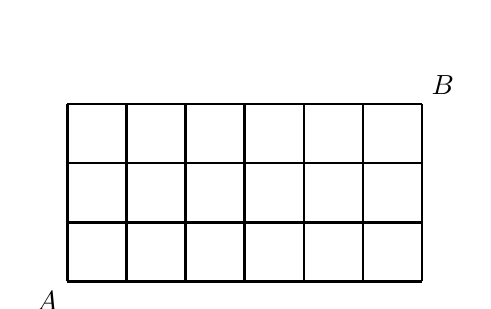
\begin{tikzpicture}[scale=0.75]
  \draw[thick] (0,0) grid (6,3);
  \node[below left] at (0,0) {$A$};
  \node[above right] at (6,3) {$B$};
\end{tikzpicture}

\vspace{0.3em}
圖 2-6
\end{center}

\indent\textbf{解}\quad 設向東走一小段（一個街口到次一街口）用 $E$ 表示，向北走一小段用 $N$ 表示，則每一種走法都是由 6 個 $E$ 及 3 個 $N$ 排列而成，例如 EEEEEENNN，因此由 (2) 式即得答案為 $9! / (6! \, 3!)$。\hfill\#

\subsubsection*{丙、環狀排列}

以上所講的都是線形排列，現在要講的是另一形狀的排列，我們將 $m$ 個不同的事物排成環狀，叫做環狀排列，在這裏我們只考慮這 $m$ 個事物的相關位置，而不計較各事物所在之實際位置，也就是說，如果將排成的環形任意轉動，所得到的結果仍表示同一環形排列，例如趙、錢、孫、李四人坐一圓桌，下列各圖形都表示同一環狀排列：

\begin{center}
\begin{tikzpicture}[scale=0.78]
  \foreach \cx/\top/\left/\bot/\right in {
    0/趙/錢/孫/李,
    4.1/李/趙/錢/孫,
    8.2/孫/李/趙/錢,
    12.3/錢/孫/李/趙
  } {
    \draw[thick] (\cx, 0) circle (1.1);
    \node[above] at (\cx, 1.1) {\top};
    \node[left] at (\cx - 1.1, 0) {\left};
    \node[below] at (\cx, -1.1) {\bot};
    \node[right] at (\cx + 1.1, 0) {\right};
  }
\end{tikzpicture}

\vspace{0.3em}
圖 2-7
\end{center}

\noindent\textbf{〔例 12〕} 若趙、錢、孫、李四人共坐一圓桌，問共有幾種坐法？

\indent\textbf{解}\quad 因為環狀排列只考慮相關位置，我們可以假想趙已坐定某一位置，再將錢、孫、李三位排入其餘三個位子，此時成為 3 中取 3 的線形排列問題，共有 $3!$ 種坐法，這也就是原來問題的答案。\hfill\#

這個問題我們也可以用另一種想法，先把環形看作線形，則 4 中取 4 的線形排列總數為 $P_4^4 = 4!$，此時每 4 種線形排列作成同一種環狀排列，例如（趙、錢、孫、李），（錢、孫、李、趙），（孫、李、趙、錢），（李、趙、錢、孫）四種排列作成同一個環狀排列（如前面圖所示），因此環狀排列總數為 $\dfrac{4!}{4} = 3!$。

由這個例子可知，對於一般情形我們也有下列結果：$m$ 個不同事物的環狀排列總數為
\begin{equation}
\frac{P_m^m}{m} = (m-1)!
\end{equation}
更進一步，如果我們考慮自 $n$ 個不同事物中任取 $m$ 個（不重複）事物的環狀排列，則總數為
\begin{equation}
\frac{P_m^n}{m} = \frac{1}{m} \frac{n!}{(n-m)!}
\end{equation}
換句話說，用 $m$ 去除線形排列總數就得到環狀排列總數，例如在例 14 (ii)\phantomsection\label{note:b5-ch2-p74-ex14}\footnote{【原書註記/校訂】：原書此處印作「例如在例 14 (ii) 中」，然前文第 70 頁土風舞男女學生間隔排成一列之題目實為〔例 11〕(ii)，此處係原書編號錯參，特此註明。}中跳土風舞時，男女學生各 5 人間隔排成一列的線形排列總數為 $2 \cdot 5! \cdot 5!$，如改為間隔的環狀排列，則總數為 $\dfrac{2 \cdot 5! \cdot 5!}{10} = 4! \, 5!$。這個問題我們也可以用第一種解法，先將男生 5 人作成環狀排列，由 (3) 式有 $(5-1)! = 4!$ 種排法，再將女生 5 人間隔插入，有 $P_5^5 = 5!$ 種排法，因此共有 $4! \cdot 5!$ 種排法，答案相同。

\noindent\textbf{〔例 13〕} 將 20 粒顏色不同的珠子串成手鐲，共有幾種串法？

\indent\textbf{解}\quad 20 中取 20 的環狀排列總數為 $(20-1)! = 19!$

但如依照一種環狀排列串好一串後，翻轉一次就表示另一反方向的環狀排列實際上表示同一種串法，因此共有 $\dfrac{19!}{2}$ 種串法。\hfill\#

\subsubsection*{習題 II-2}

\begin{enumerate}[label=\arabic*., topsep=4pt, itemsep=6pt]
  \item 某大學聯招甲組有 108 個志願，若班上 50 位同學均考甲組，所填第一志願共有多少種可能情形？
  \item 某線鐵路有 21 個站，需印製多少種車票？
  \item
  \begin{enumerate}[label=(\arabic*), topsep=2pt, itemsep=2pt]
    \item 將 100 個不同的球放入藍、白、紅三個箱中，共有多少可能放法？
    \item 試將 (1) 的問題用映射說明。
  \end{enumerate}
  \item 某次球賽共有 7 隊參加，比賽完畢排定名次，共有多少種可能情形？（設沒有相同名次）。
  \item 11 人組成的理事會中欲推選理事長、秘書、財務各一人（皆不能兼任），推選結果共有多少可能情形？
  \item
  \begin{minipage}[t]{0.68\linewidth}
  某社區巷道如右圖，\phantomsection\label{note:b5-ch2-p75-q6-quote}\footnote{【原書註記/校訂】：原書第 75 頁第 6 題「如右圖」之後印有一孤立單引號「‘」，疑為贅印或排版鉛字殘痕，此處予以刪正並附註說明。}早晨派報時由 $A$ 點進入，$B$ 點離去，需走過每條巷道，但不願重複走過同一條路，問共有幾種走法？
  \end{minipage}\hfill
  \begin{minipage}[t]{0.30\linewidth}
  \centering
  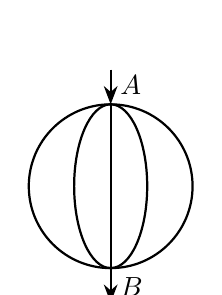
\begin{tikzpicture}[>=Stealth, scale=0.8]
    \draw[thick] (0,0) circle (1.3);
    \draw[thick] (0,0) ellipse (0.58 and 1.3);
    \draw[thick] (0,-1.3) -- (0,1.3);
    \draw[->, thick] (0, 1.85) -- (0, 1.3);
    \node[above right] at (0, 1.3) {$A$};
    \draw[->, thick] (0, -1.3) -- (0, -1.85);
    \node[below right] at (0, -1.3) {$B$};
  \end{tikzpicture}
  \end{minipage}

  \item
  \begin{minipage}[t]{0.50\linewidth}
  小明有 12 色臘筆\phantomsection\label{note:b5-ch2-p75-q7-crayon}\footnote{【原書註記/校訂】：原書作「12 色臘筆」，「臘」通「蠟」，即蠟筆。}，要將右邊的圖著色，相鄰的部分不得同色，共有幾種可能著法？
  \end{minipage}\hfill
  \begin{minipage}[t]{0.48\linewidth}
  \centering
  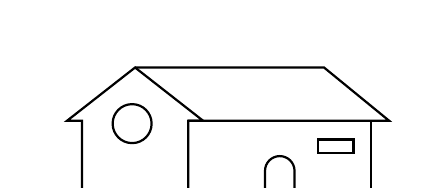
\begin{tikzpicture}[scale=0.75]
    % Ground line
    \draw[thick] (-0.6, 0) -- (6.0, 0);

    % Left front facade (with gable)
    \draw[thick] (0.3, 0) -- (0.3, 1.3) -- (0.05, 1.3) -- (1.2, 2.2) -- (2.35, 1.3) -- (2.1, 1.3) -- (2.1, 0);

    % Circular window on front gable
    \draw[thick] (1.15, 1.25) circle (0.33);

    % Right wing roof (trapezoid)
    \draw[thick] (1.2, 2.2) -- (4.4, 2.2) -- (5.5, 1.3) -- (2.1, 1.3);

    % Right wing wall
    \draw[thick] (5.2, 1.3) -- (5.2, 0);

    % Arched door on right wall
    \draw[thick] (3.4, 0) -- (3.4, 0.45) arc (180:0:0.25) -- (3.9, 0);

    % Window on right wall
    \draw[thick] (4.3, 0.75) rectangle (4.9, 0.98);
  \end{tikzpicture}
  \end{minipage}

  \item 跳土風舞時，男生 20 人，女生 16 人排成一長列，但女生不得相鄰，共有幾種可能排法？
\end{enumerate}

% ==============================================================================
% § II-3 組合
% ==============================================================================
\subsection{組合}\label{sec:b5-2-3}

\subsubsection*{甲、組合}

\noindent\textbf{定義}\quad 設 $B$ 為有限集合，$|B| = n$，對於每個自然數 $m \le n$，自 $B$ 中任取 $m$ 個不同元素作為一組（不考慮順序），叫做 $n$ 中取 $m$ 的組合．$n$ 中取 $m$ 的組合總數用 $\binom{n}{m}$ 或 $C_m^n$（或 ${}_nC_m, C(n, m)$）表示．我們約定 $n$ 中取 0，即不取，的組合總數為 1．

因為 $m$ 個不同元素的排列總數為 $P_m^m = m!$，所以在 $n$ 中取 $m$ 的一個（不重複）線形排列中，將次序變動，即可作出 $m!$ 個排列，換句話說，每 $m!$ 個排列由同一組 $m$ 個元素所作成，如不計較次序時，即為同一個 $n$ 中取 $m$ 的組合，因此我們有下列重要定理：

\medskip
\noindent\textbf{【定理 7】}$n$ 中取 $m$ 的組合總數
\begin{equation}
C_m^n = P_m^n / P_m^m = \frac{n!}{(n - m)!\, m!}, \quad 0 \le m \le n. \tag{1}
\end{equation}
有了這個定理，我們可以直接計算組合總數，\hfill $\#$

\medskip
\noindent 例如
\[
C_2^5 \phantomsection\label{note:b5-ch2-p75-eq}\footnote{【原書註記/校訂】：原書此處印為「$C_2^5 ==$」，多出一個等號，茲更正為「$C_2^5 =$」．} = \frac{5!}{(5 - 2)!\, 2!} = \frac{5!}{3!\, 2!} = \frac{5 \cdot 4}{2} = 10
\]
\[
C_5^5 = C_0^5 = 1
\]
前節中的若干重複排列問題也可以用組合方法來解，例如在論例 6 中插班生 10 人分入智、仁、勇三班的問題，我們先自 10 中取 2 分入智班，總數為 $C_2^{10}$，再在其餘 8 人中取 5 分入仁班，總數為 $C_5^8$，最後 3 人則分入勇班，因此共有
\[
C_2^{10} \cdot C_5^8 = \frac{10!}{(10 - 2)!\, 2!} \cdot \frac{8!}{(8 - 5)!\, 5!} = \frac{10!}{2!\, 5!\, 3!}
\]
種分配方法，在論例 7 (iii) 中的走法問題，自 $A$ 到 $B$ 共走九小段，向東 6\phantomsection\label{note:b5-ch2-p76-east6}\footnote{【原書註記/校訂】：原書印作「向東段及向北 3 段」，漏印「6」，茲據前文「共走九小段」及後文「考慮那 6 段向東走」校訂補正為「向東 6 段及向北 3 段」．} 段及向北 3 段，我們只要考慮那 6 段向東走，就成為 9 中取 6 的組合問題，因此走法總數為
\[
C_6^9 = \frac{9!}{(9 - 6)!\, 6!} = \frac{9!}{3!\, 6!}
\]
由 (1) 式的形狀，我們顯然有下列關係：

\medskip
\noindent\textbf{【系理】}對於 $0 \le m \le n$，下列關係成立：
\begin{equation}
\binom{n}{m} = \binom{n}{n - m} \quad (\text{即 } C_m^n = C_{n-m}^n) \tag{2}
\end{equation}

設 $B = \{b_1, b_2, \ldots, b_n\}$，由 $B$ 中任取 $m$ 個不同元素構成 $B$ 的一個子集，就是一個 $n$ 中取 $m$ 的組合，如果令 $C = \{0, 1\}$，考慮 $B$ 到 $C$ 的映射．恰好將 $B$ 中 $m$ 個元素對應到 1 的映射實際上也是一個 $n$ 中取 $m$ 的組合，此外如將 $m$ 個相同的球，放入 $n$ 個不同的箱子，但每箱至多一個，這也與 $n$ 中取 $m$ 的組合有同樣意義，總結這一段的討論我們寫成下列定理．

\medskip
\noindent\textbf{【定理 8】}設 $0 \le m \le n$，有限集合 $B$ 中元素個數為 $|B| = n$\phantomsection\label{note:b5-ch2-p76-thm8-dots}\footnote{【原書註記/校訂】：原書作「$|B| = n$，… 及 $C = \{0, 1\}$」，此處「…」為原書原文，疑為承接前段定義或排版留存之省略號．}，\dots 及 $C = \{0, 1\}$，則下列各事項在本質上具有相同的意義：
\begin{enumerate}[label=(\roman*), topsep=2pt, itemsep=4pt]
  \item $n$ 中取 $m$ 的組合．
  \item $B$ 中含 $m$ 個元素的子集．
  \item $B$ 到 $C$ 的映射，恰好將 $B$ 中 $m$ 個元素對應到 1．
  \item 將 $m$ 個相同的球放入 $n$ 個不同的箱子，但每箱至多一個．\hfill $\#$
\end{enumerate}

由 §II-1 定理 2 我們知道 $B$ 到 $C$ 的映射總數為 $|C^B| = |C|^n = 2^n$\phantomsection\label{note:b5-ch2-p77-cb}\footnote{【原書註記/校訂】：原書此處印作「$|C^B| = |C^n| = 2^n \mid$」，其中「$|C^n|$」應為「$|C|^n$」（映射集合之勢），末尾之豎線「$\mid$」疑為標點或排版雜點，茲補註說明．}，根據每個映射可取出一個 $B$ 的子集，即對應到 1 的各元素所成的子集，根據恆等於 0 的映射一個元素都不取，即得到空集合 $\phi$，這樣不難看出 $B$ 中所有子集（空集合在內）的總數就等於 $B$ 到 $C$ 的映射總數，我們將 $B$ 的所有子集構成的集合用 $\mathscr{P}(B)$ 表示，亦即
\[
\mathscr{P}(B) = \{X \mid X \subset B\}
\]
我們有
\begin{equation}
|\mathscr{P}(B)| = |C^n| = 2^n \tag{3}\phantomsection\label{note:b5-ch2-p77-pn}\footnote{【原書註記/校訂】：原書式 (3) 印刷為「$|\mathscr{P}(B)| = |C^n| = 2^n$」，若視映射集合為笛卡兒積 $C^n = C \times \cdots \times C$，其勢記為 $|C^n|$；亦即 $|C|^n = 2^n$．}
\end{equation}
另一方面，由定理 8 我們知道 $B$ 中含 $m$ 個元素的子集個數等於 $n$ 中取 $m$ 的組合個數 $C_m^n$，我們將 $m$ 自 0 至 $n$ 變動，也可以算出 $B$ 的子集總數，因而得到下列推論．

\medskip
\noindent\textbf{【系理】}
\begin{equation}
2^n = \binom{n}{0} + \binom{n}{1} + \cdots + \binom{n}{n} = \sum_{m=0}^n \binom{n}{m} \tag{4}
\end{equation}

\medskip
\noindent\textbf{【系理】}
\[
\binom{m}{k} = \binom{m-1}{k} + \binom{m-1}{k-1}
\]

\noindent\textbf{證明}\quad
\begin{align*}
\binom{m-1}{k} + \binom{m-1}{k-1} &= \frac{(m-1)!}{k!\, (m-k-1)!} + \frac{(m-1)!}{(k-1)!\, (m-k)!} \\
&= \frac{(m-1)!}{k!\, (m-k)!} (m - k + k) \\
&= \binom{m}{k}
\end{align*}
（這個式子實際上是二項係數的關係，在下一節二項定理中還會談到）．

下面我們舉個組合問題的有趣例子．\hfill $\#$

\medskip
\noindent\textbf{〔例 14〕}
\begin{enumerate}[label=(\roman*), topsep=2pt, itemsep=4pt]
  \item 在平面上任取 $n$ 個點，沒有三點共線，這 $n$ 個點決定多少根直線？
  \item[] \textbf{解}\quad $n$ 點中任取兩點決定一直線，故共決定 $C_2^n$ 條直線．
  \item 以這 $n$ 點中任三點為頂點作三角形，可作多少個三角形？
  \item[] \textbf{解}\quad 可作三角形總數為 $C_3^n$．
  \item 在平面上任取 $n$ 條直線，其中任意兩條不平行，任意三條不共點，這 $n$ 條直線共有多少交點？
  \item[] \textbf{解}\quad 每兩條不平行直線有一交點，故共有 $C_2^n$ 個交點．\hfill $\#$
\end{enumerate}

\medskip
\noindent\textbf{〔例 15〕}打橋牌所用的紙牌共 52 張（分為黑桃、紅心、方塊、梅花四種花色，每種 13 張，點數不同），問
\begin{enumerate}[label=(\roman*), topsep=2pt, itemsep=4pt]
  \item 發出一副牌（13 張）有多少種可能情形？
  \item 發出一局牌（4 副）有多少種可能情形？
\end{enumerate}
\noindent\textbf{解}
\begin{enumerate}[label=(\roman*), topsep=2pt, itemsep=4pt]
  \item 一副牌的可能情形有
  \[
  C_{13}^{52} = \frac{52!}{13!\, 39!} = 635{,}013{,}559{,}600 \text{ 種}
  \]
  \item 分到東家的牌有 $C_{13}^{52}$ 種可能情形．
  \begin{align*}
  \text{南家的牌有 } C_{13}^{52-13} &= C_{13}^{39} \text{ 種可能情形．} \\
  \text{西家的牌有 } C_{13}^{39-13} &= C_{13}^{26} \text{ 種可能情形．} \\
  \text{北家的牌有 } C_{13}^{26-13} &= C_{13}^{13} \text{ 種可能情形．}
  \end{align*}
  因而共有 $C_{13}^{52} \cdot C_{13}^{39} \cdot C_{13}^{26} \cdot C_{13}^{13}$
  \begin{align*}
  &= \frac{52!}{(52-13)!\, 13!} \frac{(52-13)!}{(39-13)!\, 13!} \frac{(39-13)!}{(26-13)!\, 13!} \frac{13!}{13!} \\
  &= \frac{52!}{(13!)^4} \text{ 種可能情形．}
  \end{align*}
\end{enumerate}

\medskip
\noindent\textbf{〔例 16〕}某次球賽共有 10 隊參加．
\begin{enumerate}[label=(\roman*), topsep=2pt, itemsep=4pt]
  \item 若採單循環制（任意兩隊都要比賽一場），要比賽多少場？
  \item 若採淘汰制，初賽每隊賽一次，共賽五場，共有多少種排法？
\end{enumerate}
\noindent\textbf{解}
\begin{enumerate}[label=(\roman*), topsep=2pt, itemsep=4pt]
  \item 這是 10 中取 2 的組合問題，所以一共要比賽
  \[
  C_2^{10} = \frac{10!}{(10-2)!\, 2!} = \frac{10 \cdot 9}{2} = 45 \text{ 場．}
  \]
  \item 這個問題比較複雜，不能直接用公式，我們可以設想自 10 隊中任取 2 隊賽第一場，有 $C_2^{10}$ 種取法，自其餘 8 隊中任取 2 隊賽第二場，有 $C_2^8$ 種取法，再自其餘 6 隊中任取 2 隊賽第三場，有 $C_2^6$ 種取法，再自其餘 4 隊中任取 2 隊賽第四場，有 $C_2^4$ 種取法；最後餘 2 隊賽第五場，因此排法總數為
  \[
  C_2^{10} \cdot C_2^8 \cdot C_2^6 \cdot C_2^4 \cdot C_2^2 = \frac{10!}{(2!)^5}
  \]
  如果我們只考慮各場比賽雙方球隊，不考慮比賽場次，則排法總數為
  \[
  \frac{1}{P_5^5} \frac{10!}{(2!)^5} = \frac{1}{5!} \frac{10!}{(2!)^5} = 9 \cdot 7 \cdot 5 \cdot 3 \cdot 1 = 945. \hfill \#
  \]
\end{enumerate}

這個答案也可以用下述比較簡單的方法推得：在 10 隊中任意取定一隊，則此隊之對手有 9 種選法；其次在其餘 8 隊中任意取定一隊，其對手有 7 種選法；再在其餘 6 隊中任意取定一隊，其對手有 5 種選法；再在其餘 4 隊中任意取定一隊，其對手有 3 種選法；最後剩下兩隊互為對手，因此亦得 $9 \cdot 7 \cdot 5 \cdot 3 \cdot 1$ 種排法．

\medskip
\noindent\textbf{【論例 8】}
\begin{enumerate}[label=(\roman*), topsep=2pt, itemsep=4pt]
  \item 下面左圖中有多少個矩形？
\end{enumerate}

\begin{figure}[H]
\centering
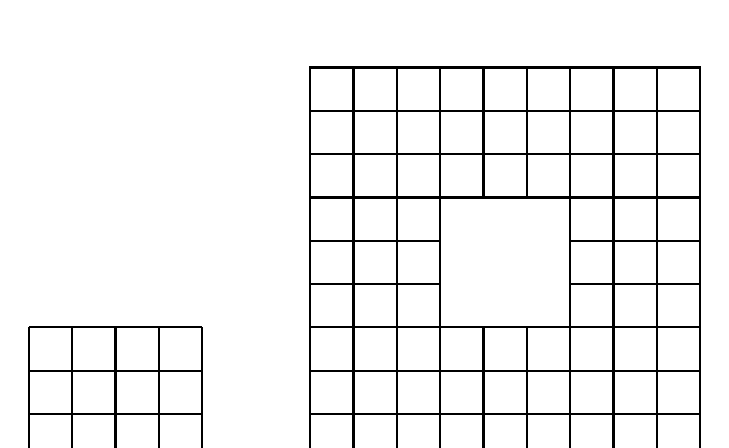
\begin{tikzpicture}[scale=0.55]
  % Left figure: 4 columns x 3 rows
  \draw[step=1cm, black, thick] (0, 0) grid (4, 3);
  
  % Right figure: 9 columns x 9 rows, central 3x3 hole
  \begin{scope}[xshift=6.5cm]
    \draw[black, thick] (0, 0) rectangle (9, 9);
    \draw[black, thick] (3, 3) rectangle (6, 6);
    % 8 sub-grids of 3x3
    \draw[step=1cm, black, thick] (0, 0) grid (3, 3);
    \draw[step=1cm, black, thick] (3, 0) grid (6, 3);
    \draw[step=1cm, black, thick] (6, 0) grid (9, 3);
    \draw[step=1cm, black, thick] (0, 3) grid (3, 6);
    \draw[step=1cm, black, thick] (6, 3) grid (9, 6);
    \draw[step=1cm, black, thick] (0, 6) grid (3, 9);
    \draw[step=1cm, black, thick] (3, 6) grid (6, 9);
    \draw[step=1cm, black, thick] (6, 6) grid (9, 9);
  \end{scope}
\end{tikzpicture}
\caption*{圖 2-8}
\label{fig:b5-2-8}
\end{figure}

\begin{enumerate}[label=(\roman*), resume, topsep=2pt, itemsep=4pt]
  \item 上面右圖中又有多少個矩形？
\end{enumerate}
\noindent\textbf{解}
\begin{enumerate}[label=(\roman*), topsep=2pt, itemsep=4pt]
  \item 因為圖中矩形係由二橫線與二直線所圍成，而二橫線之取法有 $C_2^4$ 種，二直線之取法有 $C_2^5$ 種，因此
  \[
  C_2^4 \cdot C_2^5 = 60 \text{ 個矩形．}
  \]
  \item 不包含中央方塊者有 $4 C_2^4 \cdot C_2^{10} - 4 C_2^4 \cdot C_2^4 = 936$ 個
  \begin{align*}
  \text{包含中央方塊者有 } C_1^4 \cdot C_1^4 \cdot C_1^4 \cdot C_1^4 &= 4^4 = 256 \text{ 個} \\
  \text{二者共有 } 936 + 256 &= 1192 \text{ 個．} \tag*{\#}
  \end{align*}
\end{enumerate}

% ==============================================================================
% 乙、重複組合
% ==============================================================================
\subsubsection*{乙、重複組合}

以上討論均為不重複組合，例如將 $m$ 個相同的球，放入 $n$ 個不同的箱子，但限制每箱至多一個，現在我們考慮重複組合．

\medskip
\noindent\textbf{定義}\quad 設有限集合 $B$ 中元素個數為 $|B| = n$，自 $B$ 中任取 $m$ 個元素（可以重複選取）成為一組，叫做 $n$ 中取 $m$ 的重複組合， $n$ 中取 $m$ 的重複組合總數用 $H_m^n$（或 ${}_n H_m, H(n, m)$）表示．

$m = 0$ 時我們仍約定 $H_0^n = 1$；$m = 1$ 時顯然 $H_1^n = C_1^n = n$．

$m = 2$ 時，我們將所取各種組合分為兩類來討論，一類是自 $n$ 個不同元素中重複取兩個相同元素，有 $n$ 種取法；另一類是自 $n$ 個不同元素中取兩個不同元素，即成為 $n$ 中取 2 的不重複組合，有 $C_2^n$ 種取法，因此 $n$ 中取 2 的重複組合總數為
\[
H_2^n = n + C_2^n = n + \frac{n(n-1)}{2} = \frac{(n+1)n}{2}
\]

$m = 3$ 時，取三個全同元素的組合總數為 $n$，取三個元素，其中兩個相同的組合總數為 $n(n-1)$，取三個不同元素的組合總數為 $C_3^n$，因此
\begin{align*}
H_3^n &= n + n(n-1) + C_3^n \\
&= \frac{(n+2)(n+1)n}{6}
\end{align*}

由以上的計算，我們看出當 $m$ 愈大時，這種方法的分類就愈多，計算就愈複雜．

下面我們用另一種想法，來導出 $H_m^n$ 的一般公式，令集合 $B = \{b_1, \ldots, b_n\}$，並設一個任意的 $n$ 中取 $m$ 的重複組合，自 $B$ 中取出 $m_1$ 個 $b_1, m_2$ 個 $b_2, \ldots, m_k$ 個 $b_k, \ldots, m_n$ 個 $b_n$ ($m_1, \ldots, m_n$ 皆為非負整數且 $m_1 + \cdots + m_n = m$)，我們可將所取的元素按照足標次序及重複個數排列如下：
\[
\underbrace{b_1 \cdots\cdots b_1}_{m_1 \text{ 個}} \quad \underbrace{b_2 \cdots\cdots b_2}_{m_2 \text{ 個}} \cdots\cdots\cdots\cdots\cdots \underbrace{b_n \cdots\cdots b_n}_{m_n \text{ 個}}
\]
為了分隔清楚起見，我們再用 $n-1$ 個短豎把這個有限序列分成 $n$ 個小段：
\[
\underbrace{b_1 \cdots\cdots b_1}_{m_1 \text{ 個}} \;\Big|\; \underbrace{b_2 \cdots\cdots b_2}_{m_2 \text{ 個}} \;\Big|\; \cdots\cdots \;\Big|\; \underbrace{b_n \cdots\cdots b_n}_{m_n \text{ 個}},
\]
如果 $m_k = 0$ 時，則那一小段中就沒有元素，在這樣分隔之下，在第一小段中的元素都是 $b_1$，在第二小段中的元素都是 $b_2 \cdots$，在第 $n$ 小段（即最後一段）中的元素都是 $b_n$，我們發現，如果把其中各元素的足標省略，寫成下列形狀：
\[
\underbrace{b \cdots\cdots b}_{m_1} \;\Big|\; \underbrace{b \cdots\cdots b}_{m_2} \;\Big|\; \cdots\cdots \;\Big|\; \underbrace{b \cdots\cdots b}_{m_n},
\]
仍然可以明確表示原來所取的組合，為了討論方便，我們更進一步，把 $b$ 改用 1 代表，把短豎 $\mid$ 改用 0 代表，而得到下列形狀的序列．
\[
\underbrace{1 \cdots\cdots 1}_{m_1} \;0\; \underbrace{1 \cdots\cdots 1}_{m_2} \;0 \cdots\cdots\cdots 0\; \underbrace{1 \cdots\cdots 1}_{m_n}
\]
換句話說，一個 $n$ 中取 $m$ 的重複組合可以用 $m$ 個 1 及 $n-1$ 個 0 排成的序列來表示．反之每個這樣的序列都表示一個 $n$ 中取 $m$ 的重複組合，例如
\[
1110100110001111
\]
這個序列中有 10 個 1 及 6 個 0，表示一個 7 中取 10 的重複組合：
\[
b_1\, b_1\, b_1\, b_2\, b_4\, b_4\, b_7\, b_7\, b_7\, b_7
\]
要計算 $n$ 中取 $m$ 的重複組合總數 $H_m^n$，現在只要來計算由 $m$ 個 1 及 $n-1$ 個 0 所作成的有限序列總數，這種有限序列的長度為 $m+n-1$，在其中取定 $m$ 個位置以 1 填入，而在其餘 $n-1$ 個位置以 0 填入，就得到一個確定的序列，我們把序列中的 $m+n-1$ 個位置編成 $1, 2, \ldots, m+n-1$ 號碼，在其中任取 $m$ 個位置就等於在集合 $\{1, 2, \ldots, m+n-1\}$ 中取 $m$ 個不同的數字，這是一個 $m+n-1$ 中取 $m$ 的（不重複）組合，因此總數為 $C_m^{m+n-1}$，這也就等於 $n$ 中取 $m$ 的重複組合總數，我們把上述結果寫成下列定理：

\medskip
\noindent\textbf{【定理 9】}設 $n$ 為自然數，$m$ 為非負整數，則 $n$ 中取 $m$ 的重複組合總數
\begin{equation*}
H_m^n = C_m^{m+n-1} = \frac{(m+n-1)!}{m!\, (n-1)!}
\end{equation*}

\medskip
\noindent\textbf{〔例 17〕}
\begin{enumerate}[label=(\roman*), topsep=2pt, itemsep=4pt]
  \item 同時擲兩顆骰子，有多少種可能結果？
  \item 如同時擲六顆骰子，又有多少種可能結果？
\end{enumerate}
\noindent\textbf{解}
\begin{enumerate}[label=(\roman*), topsep=2pt, itemsep=4pt]
  \item 這是 6 中取 2 的重複組合問題，有
  \[
  H_2^6 = C_2^{2+6-1} = \frac{7!}{2!\, 5!} = 21 \text{ 種可能情形．}
  \]
  實際上可能出現的情形如下圖：
  \[
  \begin{array}{cccccc}
  (1, 1), & (1, 2), & (1, 3), & (1, 4), & (1, 5), & (1, 6) \\
          & (2, 2), & (2, 3), & (2, 4), & (2, 5), & (2, 6) \\
          &         & (3, 3), & (3, 4), & (3, 5), & (3, 6) \\
          &         &         & (4, 4), & (4, 5), & (4, 6) \\
          &         &         &         & (5, 5), & (5, 6) \\
          &         &         &         &         & (6, 6)
  \end{array}
  \]
  \item 這是 6 中取 6 的重複組合，可能出現情形有
  \[
  H_6^6 = \frac{(6+6-1)!}{6!\, (6-1)!} = \frac{11!}{6!\, 5!} = 462 \text{ 種．} \tag*{\#}
  \]
\end{enumerate}

\medskip
\noindent\textbf{【論例 9】}
\begin{enumerate}[label=(\roman*), topsep=2pt, itemsep=4pt]
  \item $n$ 個變數的方程式
  \[
  x_1 + x_2 + \cdots + x_n = m \quad (m \text{ 為正整數})
  \]
  的非負整數解有多少組？
  \item 如果 $m \ge n$，上述方程式的正整數解有多少組？
\end{enumerate}
\noindent\textbf{解}
\begin{enumerate}[label=(\roman*), topsep=2pt, itemsep=4pt]
  \item 設 $S = \{b_1, \ldots, b_n\}$．其中 $b_1, \ldots, b_n$ 為 $n$ 個相異元素．如果自 $S$ 中任取 $m$ 個元素，而以 $x_i$ 表示所取元素 $b_i$ 的重複個數（$b_i$ 沒有被取到時，則 $x_i = 0$），則 $(x_1, \ldots, x_n)$ 這一組數就是方程式的一組解．因此方程式的解的個數就等於 $n$ 中取 $m$ 的重複組合總數，即 $H_m^n$．
  \item 要求的是正整數解，我們令
  \[
  y_k = x_k - 1, \quad k = 1, \ldots, n
  \]
  則原式化為
  \[
  y_1 + \cdots + y_n = m - n,
  \]
  這個方程式的非負整數解的組數為 $H_{m-n}^n$，也就是原式的正整數解的組數．
\end{enumerate}
由上例可知方程式 $x + y + z = 10$ 有 $H_{10}^3 = 66$ 組非負整數解，以及 $H_7^3 = 36$ 組正整數解．

\medskip
\noindent\textbf{〔例 18〕}
\begin{enumerate}[label=(\roman*), topsep=2pt, itemsep=4pt]
  \item 將 50 個相同的球，放在 4 個不同的箱中，有多少種放法？
  \item 某班有同學 50 人，採用不記名投票選舉幹事一人．假設有 4 位候選人，並設開票時沒有廢票，問投票的分佈有多少種可能情形？
\end{enumerate}
\noindent\textbf{解}\quad 這兩個問題在本質上相同，都是 4 中取 50 的重複組合，總數為
\[
H_{50}^4 = \frac{53!}{50!\, 3!} = \frac{53 \cdot 52 \cdot 51}{3 \cdot 2} = 23426 \tag*{\#}
\]

\medskip
\noindent\textbf{【論例 10】}如將 $(x_1 + \cdots + x_n)^m$ 展開\phantomsection\label{note:b5-ch2-p83-zhankai}\footnote{【原書註記/校訂】：原書作「展開式 $m$ 次齊次式」，疑為「展開成 $m$ 次齊次式」或「展開之 $m$ 次齊次式」，此處依文意校正為「展開成 $m$ 次齊次式」．}成 $m$ 次齊次式，問其中不同類的項有多少種（即合併同類項後有多少項）？

\noindent\textbf{解}\quad 一個任意的項 $x_1^{m_1} x_2^{m_2} \cdots x_n^{m_n}$ 可以看成一個 $n$ 中取 $m$ 的重複組合，因此不同類的項共有 $H_m^n$ 種例如 $(x + y + z)^{10}$ 的展開式中不同類的項共有 $H_{10}^3 = 66$ 種．

% ==============================================================================
% 習題 II-3
% ==============================================================================
\subsubsection*{習題 II-3}\label{sec:b5-ex2-3}

\begin{enumerate}[label=\textbf{\arabic*.}]
  \item 設 $A = \{a, b, c\}$，試求 $|\mathscr{P}(A)|$，即 $A$ 的所有子集的個數．
  \item 班上 50 位同學中派出 10 位公差整理校園，共用\phantomsection\label{note:b5-ch2-p83-gongyong}\footnote{【原書註記/校訂】：原書作「共用幾種可能派法」，「用」疑為「有」之誤．}幾種可能派法？
  \item 設 $A = \{1, 2, \ldots, 100\}$，求 $A$ 中恰含 10 個元素的子集個數．
  \item
  \begin{minipage}[t]{0.64\linewidth}
  \begin{enumerate}[label=(\arabic*)]
    \item 設街道如圖，若自 $A$ 點漫步到 $B$ 點，不必走過所有街道，但走過的不欲再走，問共有幾種走法？
    \item 如將縱向街道改為 $n$ 條，試求答案．
  \end{enumerate}
  \end{minipage}\hfill
  \begin{minipage}[t]{0.32\linewidth}
  \centering
  \vspace{0pt}
  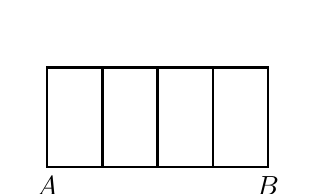
\begin{tikzpicture}[scale=0.7]
    \draw[thick] (0, 0) rectangle (4, 1.8);
    \foreach \x in {1, 2, 3} {
      \draw[thick] (\x, 0) -- (\x, 1.8);
    }
    \node[below] at (0, 0) {$A$};
    \node[below] at (4, 0) {$B$};
  \end{tikzpicture}
  \end{minipage}
  \item 試求
  \begin{enumerate}[label=(\arabic*)]
    \item $H_2^5$
    \item $H_3^3$
    \item $H_2^{100}$
  \end{enumerate}
  \item 假設班上 8 位同學去冷飲店，那裏有六種飲料供選擇，每人任點一種，共有幾種點法？（重複組合問題）
  \item 跳棋盒中有紅、黃、綠三種顏色棋子．若隨手抓出 10 個子，共有多少種可能情形？
  \item[*8.] 試證
  \begin{enumerate}[label=(\arabic*)]
    \item $H_m^n = H_{n-1}^{m+1}$
    \item $m H_m^n = n H_n^m$
  \end{enumerate}
  \item 同時擲三粒骰子時，有多少種可能結果？
  \item[*10.] 給予方程式 $u + v + w + x + y + z = 10$，問
  \begin{enumerate}[label=(\arabic*)]
    \item 有多少組非負整數解？
    \item 有多少組正整數解？
  \end{enumerate}
  \item 將一張百元大鈔換成 50 元，10 元，5 元或一元券，共有多少種換法？
\end{enumerate}

% =========================================================================
% 《高中數學實驗教材》第五冊（自然組）
% 第二章 排列組合
% §II-4 二項式定理 (Pages 84--93)
% =========================================================================

\subsection{二項式定理}\label{sec:b5-2-4}

\subsubsection*{甲、二項式定理}\label{subsec:b5-2-4-a}

如果我們將 $(x + y)^3$ 展開並合併同類項，則得
\[ (x + y)^3 = x^3 + 3x^2 y + 3xy^2 + y^3. \]
對於一般情形我們有下列定理：

\medskip
\noindent\textbf{【定理 10】（二項式定理）}\label{thm:b5-2-10}

對於任意自然數 $m$，我們有下列二項展開式
\begin{align}
(x + y)^m &= \binom{m}{0} x^m + \binom{m}{1} x^{m-1} y + \dotsb + \binom{m}{k} x^{m-k} y^k + \dotsb + \binom{m}{m} y^m \notag \\
&= \sum_{k=0}^m \binom{m}{k} x^{m-k} y^k. \label{eq:b5-2-4-1}\tag{1}
\end{align}
〔我們約定 $(x + y)^0 = 1$〕。

\medskip
\noindent\textbf{證明}\quad $(x + y)^m$ 表示 $m$ 個二項式 $x + y$ 的連乘積，如果我們只用分配律，而不用乘法交換律時，則所得到乘積形狀如下：
\begin{align*}
(x + y)^m &= (x + y)(x + y)\dotsb(x + y) \\
&= [(x + y)(x + y)][(x + y)\dotsb(x + y)] \\
&= [x(x + y) + y(x + y)][(x + y)\dotsb(x + y)] \\
&= [xx + xy + yx + yy][(x + y)\dotsb(x + y)] \\
&= xx\dotsb xx + xx\dotsb xy + xx\dotsb xyx \\
&\quad + xx\dotsb xyy + \dotsb + yy\dotsb yx + yy\dotsb yy
\end{align*}%
\phantomsection\label{note:b5-ch2-p85-expand}\footnote{【原書註記/校訂】：原書此處展開式各項印為「$xx\cdots xx + xx\cdots xy + xx\cdots xyx + xx\cdots xyy + \cdots + yy\cdots yx + yy\cdots yy$」。按依字典次序（若設 $x=0, y=1$），前四項末尾長度為 3 之排列應依序為 $xxx, xxy, xyx, xyy$；原書前二項省略至兩字元，後二項書為三字元，此處照原刊本排印並予說明。}
上式中共有 $2^m$ 項，每一項都用 $m$ 個字母構成，而且恰好照字典中的方法排列次序，由於不用乘法交換律，沒有兩項是相同的。（如將 $x$ 改為 $0$，$y$ 改為 $1$，則成為由小到大的次序，可以看得更清楚），上式中一個典型的項是由 $k$ 個 $y$ 及 $m - k$ 個 $x$ 所排成，我們不難求出由 $k$ 個 $y$ 及 $m - k$ 個 $x$ 作出的不同排列總數為 $\dbinom{m}{k}$，因此合併同類項，則 $x^{m-k} y^k$ 的係數即為 $\dbinom{m}{k}$。

\medskip
\noindent\textbf{另一證法}\quad 利用歸納法證明如下：

$m = 1$ 時 $(x + y)^1 = \dbinom{1}{0} x + \dbinom{1}{1} y$，故公式成立。假定 $m$ 也成立，利用 \S II-3 定理 8 的系理
\[ \binom{m}{k-1} + \binom{m}{k} = \binom{m+1}{k} \]
可推得 $m+1$ 時亦成立，證明如下：
\begin{align*}
(x + y)^{m+1} &= (x + y)(x + y)^m \\
&= (x + y) \left[ \binom{m}{0} x^m + \binom{m}{1} x^{m-1} y + \dotsb \right. \\
&\qquad\quad \left. + \binom{m}{k-1} x^{m-k+1} y^{k-1} + \binom{m}{k} x^{m-k} y^k + \dotsb + \binom{m}{m} y^m \right] \\
&= \binom{m}{0} x^{m+1} + \left[ \binom{m}{0} + \binom{m}{1} \right] x^m y + \dotsb \\
&\qquad\quad + \left[ \binom{m}{k-1} + \binom{m}{k} \right] x^{m-k+1} y^k + \dotsb + \binom{m}{m} y^{m+1} \\
&= \binom{m+1}{0} x^{m+1} + \binom{m+1}{1} x^m y + \dotsb \\
&\qquad\quad + \binom{m+1}{k} x^{(m+1)-k} y^k + \dotsb + \binom{m+1}{m+1} y^{m+1}.
\end{align*}

由二項定理我們看到 $m$ 中取 $k$ 的（不重複）組合總數恰好就是二項展開式第 $k+1$ 項 $\dbinom{m}{k} x^{m-k} y^k$ 的係數，所以我們就把 $\dbinom{m}{k}$，（即 $C^m_k$）也叫做\underline{二項係數}。

\medskip
\noindent\textbf{〔例 19〕}\label{ex:b5-2-19}展開下列各式
\begin{enumerate}[label=(\roman*)]
  \item $(x + y)^7$
  \item $(a + 3b)^4$
  \item $(3a + 5b)^3$
\end{enumerate}

\noindent\textbf{解}
\begin{enumerate}[label=(\roman*)]
  \item \begin{align*}
  (x + y)^7 &= \sum_{k=0}^7 \binom{7}{k} x^{7-k} y^k \\
  &= \binom{7}{0} x^7 + \binom{7}{1} x^6 y + \binom{7}{2} x^5 y^2 + \binom{7}{3} x^4 y^3 \\
  &\quad + \binom{7}{4} x^3 y^4 + \binom{7}{5} x^2 y^5 + \binom{7}{6} x y^6 + \binom{7}{7} y^7 \\
  &= x^7 + 7x^6 y + 21x^5 y^2 + 35x^4 y^3 \\
  &\quad + 35x^3 y^4 + 21x^2 y^5 + 7xy^6 + y^7
  \end{align*}
  \item \begin{align*}
  (a + 3b)^4 &= \binom{4}{0} a^4 + \binom{4}{1} a^3 (3b) + \binom{4}{2} a^2 (3b)^2 + \binom{4}{3} a (3b)^3 + \binom{4}{4} (3b)^4 \\
  &= a^4 + 12a^3 b + 54a^2 b^2 + 108ab^3 + 81b^4
  \end{align*}
  \item \begin{align*}
  (3a + 5b)^3 &= \binom{3}{0} (3a)^3 + \binom{3}{1} (3a)^2 (5b) + \binom{3}{2} (3a)(5b)^2 + \binom{3}{3} (5b)^3 \\
  &= 27a^3 + 135a^2 b + 225ab^2 + 125b^3 \qquad \#
  \end{align*}
\end{enumerate}

\medskip
\noindent\textbf{〔例 20〕}\label{ex:b5-2-20}求下列各式中指定項的係數：
\begin{enumerate}[label=(\roman*)]
  \item $\left(x + \dfrac{1}{x}\right)^{10}$ 中 $x^4$ 的係數。
  \item $\left(2x - \dfrac{1}{3x}\right)^9$ 中 $x^3$ 的係數。
  \item $\left(2x^2 + \dfrac{3}{x}\right)^6$ 中的常數項。
\end{enumerate}

\noindent\textbf{解}
\begin{enumerate}[label=(\roman*)]
  \item 因 $x^7 \left(\dfrac{1}{x}\right)^3 = x^4$，所求為 $\dbinom{10}{3} = 120$
  \item 因 $x^6 \left(\dfrac{1}{x}\right)^3 = x^3$，所求 $\dbinom{9}{3} 2^6 \cdot \left(-\dfrac{1}{3}\right)^3 = -\dfrac{1792}{9}$
  \item 因 $(x^2)^2 \left(\dfrac{1}{x}\right)^4 = 1$，所求為 $\dbinom{6}{4} \cdot 2^2 \cdot 3^4 = 4860$
\end{enumerate}

\medskip
\noindent\textbf{〔例 21〕}\label{ex:b5-2-21}擲硬幣 10 次，有多少種情形得到 6 次正面與 4 次背面？

\noindent\textbf{解}\quad 如將正面記作 $x$，背面記作 $y$，則所求答案即為 $(x + y)^{10}$ 中 $x^6 y^4$ 的係數，等於 $\dbinom{10}{4} = 210$

\bigskip
如果在 (1) 式中令 $x = 1$，則得下列展開式
\begin{equation}
(1 + y)^m = \sum_{k=0}^m \binom{m}{k} y^k. \label{eq:b5-2-4-2}\tag{2}
\end{equation}
例如
\begin{align*}
(1 + t)^6 &= \binom{6}{0} + \binom{6}{1} t + \binom{6}{2} t^2 + \binom{6}{3} t^3 + \binom{6}{4} t^4 + \binom{6}{5} t^5 + \binom{6}{6} t^6 \\
&= 1 + 6t + 15t^2 + 20t^3 + 15t^4 + 6t^5 + t^6,
\end{align*}
如果在 (2) 式中再令 $y = 1$ 及 $-1$，則得
\begin{align*}
2^m &= \sum_{k=0}^m \binom{m}{k} = \binom{m}{0} + \binom{m}{1} + \dotsb + \binom{m}{m} \\
0 &= \sum_{k=0}^m (-1)^k \binom{m}{k} = \binom{m}{0} - \binom{m}{1} + \binom{m}{2} - \dotsb + (-1)^m \binom{m}{m}
\end{align*}
由 \S II-3 組合的討論我們知道 $\dbinom{m}{k}$ 滿足下列關係式
\begin{equation}
\binom{m}{k} = \binom{m-1}{k} + \binom{m-1}{k-1} \label{eq:b5-2-4-3}\tag{3}
\end{equation}
這個式子可以簡單的解釋如下：在 $m$ 個元素中指定一個元素，例如 $b_m$，則 $m$ 中取 $k$ 的（不重複）組合中不含 $b_m$ 的總數為 $\dbinom{m-1}{k}$，而含 $b_m$ 的總數為 $\dbinom{m-1}{k-1}$，二者合計為 $\dbinom{m-1}{k} + \dbinom{m-1}{k-1}$，即為 $m$ 中取 $k$ 的（不重複）組合總數，在二項定理中如果將 $(x+y)^m$ 中的因式 $(x+y)^{m-1}$ 先展開，然後再乘 $(x+y)$，則亦得 (3) 式。

我們寫出 $m = 0, 1, 2, \dots\dots$ 的各個二項展開式
\begin{center}
\begin{tabular}{rcc}
$(x + y)^0 =$ & $1$ \\
$(x + y)^1 =$ & $x + y$ \\
$(x + y)^2 =$ & $x^2 + 2xy + y^2$ \\
$(x + y)^3 =$ & $x^3 + 3x^2 y + 3xy^2 + y^3$ \\
$(x + y)^4 =$ & $x^4 + 4x^3 y + 6x^2 y^2 + 4xy^3 + y^4$ \\
$(x + y)^5 =$ & $x^5 + 5x^4 y + 10x^3 y^2 + 10x^2 y^3 + 5xy^4 + y^5$ \\
$\dots\dots$ & $\dots\dots$
\end{tabular}
\end{center}
如果我們將上面的 $x, y$ 省略，只列出各項係數，就得到二項係數的\underline{巴斯卡} (Pascal) \underline{三角形}：

\begin{center}
\begin{tikzpicture}[x=0.8cm, y=0.65cm]
  \node at (0, 0) {$1$};
  \node at (-0.6, -1) {$1$};
  \node at (0.6, -1) {$1$};
  \node at (-1.2, -2) {$1$};
  \node at (0, -2) {$2$};
  \node at (1.2, -2) {$1$};
  \node at (-1.8, -3) {$1$};
  \node at (-0.6, -3) {$3$};
  \node at (0.6, -3) {$3$};
  \node at (1.8, -3) {$1$};
  \node at (-2.4, -4) {$1$};
  \node at (-1.2, -4) {$4$};
  \node at (0, -4) {$6$};
  \node at (1.2, -4) {$4$};
  \node at (2.4, -4) {$1$};
  \node at (-3.0, -5) {$1$};
  \node at (-1.8, -5) {$5$};
  \node at (-0.6, -5) {$10$};
  \node at (0.6, -5) {$10$};
  \node at (1.8, -5) {$5$};
  \node at (3.0, -5) {$1$};
  \node at (-3.0, -6) {$\dots\dots$};
  \node at (0, -6) {$\dots\dots$};
  \node at (3.0, -6) {$\dots\dots$};
\end{tikzpicture}
\end{center}

這個三角形的邊緣都是 1，而內部的數都是它的左上方及右上方二數的和（就是 (3) 式）所以巴斯卡三角形就是 (3) 式中的一種具體的表示方法，利用巴斯卡三角形我們能夠直接寫出一些二項展開式，而得到不少方便。

\subsubsection*{乙、多項式定理}\label{subsec:b5-2-4-b}

利用二項式定理，我們可以討論多項式
\[ (x_1 + \dotsb + x_n)^m \]
的展開，首先我們考慮三個變數的情形：
\[ (x + y + z)^m = [x + (y + z)]^m \]
\begin{align}
&= \sum_{k=0}^m \binom{m}{k} x^{m-k} (y + z)^k \notag \\
&= \sum_{k=0}^m \binom{m}{k} x^{m-k} \left[ \sum_{j=0}^k \binom{k}{j} y^{k-j} z^j \right] \notag \\
&= \sum_{k=0}^m \sum_{j=0}^k \binom{m}{k} \binom{k}{j} x^{m-k} y^{k-j} z^j \label{eq:b5-2-4-4}\tag{4}
\end{align}%
\phantomsection\label{note:b5-ch2-p90-binom}\footnote{【原書註記/校訂】：原書第 90 頁 (4) 式中雙重求和號內印作「$\binom{n}{k} \binom{k}{j}$」，其中「$\binom{n}{k}$」顯係「$\binom{m}{k}$」之印刷訛誤，此處逕予更正。}
現在我們引用一個新的符號，定義
\[ \binom{m}{m-k, k-j, j} = \binom{m}{k} \binom{k}{j} = \frac{m!}{(m-k)!(k-j)!j!} \]
如令 $m - k = P_1$，$k - j = P_2$，$j = P_3$，則 $P_1 + P_2 + P_3 = m$，而
\[ \binom{m}{P_1, P_2, P_3} = \frac{m!}{P_1! P_2! P_3!} \]
將新符號代入 (4) 式，即得
\begin{align*}
(x + y + z)^m &= \sum_{\substack{P_1 + P_2 + P_3 = m \\ 0 \le P_1, P_2, P_3 \le m}} \binom{m}{P_1, P_2, P_3} x^{P_1} y^{P_2} z^{P_3} \\
&= \sum_{\substack{P_1 + P_2 + P_3 = m \\ 0 \le P_1, P_2, P_3 \le m}} \frac{m!}{P_1! P_2! P_3!} x^{P_1} y^{P_2} z^{P_3}
\end{align*}

\medskip
\noindent\textbf{【論例 11】}\label{ex:b5-2-disc11}將 $(x + y + z)^4$\phantomsection\label{note:b5-ch2-p90-ex11-typo}\footnote{【原書註記/校訂】：原書第 90 頁此處題目印為「將 $(x+y+y)^4$ 展開」，顯係「$(x+y+z)^4$」之排印訛誤，依解答逕予更正。} 展開

\noindent\textbf{解}
\begin{align*}
(x + y + z)^4 &= \sum_{\substack{P_1 + P_2 + P_3 = 4 \\ 0 \le P_1, P_2, P_3 \le 4}} \frac{4!}{P_1! P_2! P_3!} x^{P_1} y^{P_2} z^{P_3} \\
&= (x^4 + y^4 + z^4) + 4(x^3 y + y^3 x + x^3 z + z^3 x + y^3 z + z^3 y) \\
&\quad + 6(x^2 y^2 + y^2 z^2 + z^2 x^2) + 12(x^2 yz + xy^2 z + xyz^2) \qquad \#
\end{align*}%
\phantomsection\label{note:b5-ch2-p90-ex11-y4}\footnote{【原書註記/校訂】：原書第 90 頁此式解答第一括弧內印作「$(x^4 + x^4 + z^4)$」，其中第二項「$x^4$」顯係「$y^4$」之誤，此處逕予更正。}%
（由論例 10\phantomsection\label{note:b5-ch2-p90-disc10}\footnote{【原書註記/校訂】：原書此處引「由論例 10 知上式有 $H_4^3 = 15$ 個不同類項」，係指前節（\S II-3 重複組合）中討論多元一次方程式非負整數解或多項式展開項數之論例。} 知上式有 $H_4^3 = 15$ 個不同類項）

\medskip
\noindent\textbf{【例 22】}\label{ex:b5-2-22}求 $(x - 3y + z)^8$ 中 $x^2 y^3 z^3$ 的係數

\noindent\textbf{解}\quad $m = 8,\; P_1 = 2,\; P_2 = 3,\; P_3 = 3$，則
\[ \binom{8}{2, 3, 3} = \frac{8!}{2! 3! 3!} = 560 \]
$x^2 y^3 z^3$ 的係數為 $560 \cdot (-3)^3 = -15120$ \hfill \#

\bigskip
對於 $n$ 個變數的情形，我們有下列定理。

\medskip
\noindent\textbf{【定理 11】（多項式定理）}\label{thm:b5-2-11}
\begin{equation}
(x_1 + x_2 + \dotsb + x_n)^m = \sum_{\substack{P_1 + \dotsb + P_n = m \\ 0 \le P_1, \dots, P_n \le m}} \binom{m}{P_1, \dots, P_n} x_1^{P_1} x_2^{P_2} \dotsb x_n^{P_n} \label{eq:b5-2-4-5}\tag{5}
\end{equation}%
\phantomsection\label{note:b5-ch2-p91-eq5}\footnote{【原書註記/校訂】：原書正文於後續推導中稱「如在 (5) 中令 $x_1 = x_2 = \cdots = x_n = 1$」，然此處定理陳述式右端漏印編號標籤「(5)」，此處依文意補上編號 (5)。}
式中 $\dbinom{m}{P_1, \dots, P_n} = \dfrac{m!}{P_1! P_2! \dotsm P_n!}$

\medskip
\noindent\textbf{證明}\quad $x_1^{P_1} x_2^{P_2} \dots\dots x_n^{P_n}$ 的係數等於 $P_1$ 個 $x_1$，$P_2$ 個 $x_2$，$\dots\dots$，$P_n$ 個 $x_n$，共 $P_1 + \dots\dots + P_n = m$ 個元素的排列總數，我們先將這 $m$ 個元素想成互異的，則排列個數為 $P^m_m = m!$，因 $P_1$ 個 $x_1$ 是相同，故應用 $P_1!$\phantomsection\label{note:b5-ch2-p91-p1}\footnote{【原書註記/校訂】：原書此處印作「故應用 $P!$ 去除」，漏印足標 1，此處更正為「$P_1!$」。} 去除，依此類推，所以要求的係數等於
\[ \frac{m!}{P_1! P_2! \dotsm P_n!}\phantomsection\label{note:b5-ch2-p91-pm}\footnote{【原書註記/校訂】：原書此處分母末項印作「$P_m!$」，依變數個數 $n$ 應為「$P_n!$」，此處逕予更正。} \]

如在 (5) 中令 $x_1 = x_2 = \dotsb = x_n = 1$，則得
\[ n^m = \sum_{\substack{P_1 + \dotsb + P_n = m \\ 0 \le P_1, \dots, P_n \le m}} \binom{m}{P_1, \dots, P_n}, \]
上式左邊為 $n$ 中取 $m$ 的重複排列總數，右邊\phantomsection\label{note:b5-ch2-p91-right}\footnote{【原書註記/校訂】：原書此處印為「左邊的各項則為」，與前半句「上式左邊為」重複，依文意右端各項乃就選取個數分類，故「左邊」顯為「右邊」之筆誤，此處逕予更正為「右邊」。}的各項則為 $n$ 中取 $m$ 的重複排列（但限定 $P_1$ 個 $x_1$，$\dots\dots$ $P_n$ 個 $x_n$）總數。

\medskip
\noindent\textbf{【例 23】}\label{ex:b5-2-23}擲骰子 6 次，問有多少種情形得到兩個四，兩個五及兩個六？

\noindent\textbf{解}\quad 令 $x_k$ 表示出現 $k$ 點的情形，則所求即為 $(x_1 + x_2 + x_3 + x_4 + x_5 + x_6)^6$ 中 $x_4^2 x_5^2 x_6^2$ 的係數，等於 $\dfrac{6!}{2! 2! 2!} = 90$

\medskip
\noindent\textbf{作業 1}\label{hw:b5-2-1}求 $(x + y + z + t)^8$ 中 $x^3 y z^2 t^2$ 及 $x y^6 t$ 的係數。

\medskip
\noindent\textbf{〔例 24〕}\label{ex:b5-2-24}設 $m, n$ 皆為自然數，試證
\[ (n^2)! / (n!)^{n+1} \text{ 及 } (mn)! / (m!)^n n! \text{ 皆為整數。} \]

\noindent\textbf{證明}\quad 因為 $n^2 = \underbrace{n + \dotsb + n}_{n\text{ 個}}$，如將 $n^2$ 個不同的東西分入 $n$ 個相同的箱子，限定每箱恰好 $n$ 個，則總數即為
\[ \frac{1}{n!} \binom{n^2}{n, \dots, n} = (n^2)! / (n!)^{n+1}. \]
所以 $(n^2)! / (n!)^{n+1}$ 為整數。

$(mn)! / (m!)^n n!$ 則恰為 $mn$ 個不同的東西分入 $n$ 個同樣的箱子，每箱恰好 $m$ 個的分法總數，所以也是整數。

\subsubsection*{習題 II-4}\label{sec:b5-ex2-4}

\begin{enumerate}[label=\arabic*.]
  \item 將 $(x + y)^m$ 展開，共有多少不同類的項？
  \item 展開下列各式：
  \begin{enumerate}[label=(\arabic*)]
    \item $(x + y)^3$
    \item $(x - 2)^5$
    \item $\left(2x + \dfrac{y}{2}\right)^4$
  \end{enumerate}
  \item 求下列各式中指定項的係數
  \begin{enumerate}[label=(\arabic*)]
    \item $\left(x + \dfrac{1}{x}\right)^{10}$ 中 $x^6$ 的係數
    \item $\left(2x - \dfrac{1}{3x}\right)^8$ 中的常數項
    \item $\left(2x^2 + \dfrac{3}{x}\right)^5$ 中 $x^3$ 的係數\phantomsection\label{note:b5-ch2-p92-q3-3}\footnote{【原書註記/校訂】：原書第 92 頁此小題印為「$\left(2x^2 + \frac{3}{x}\right)^5$ 中 $x^3$ 的係數」。按其一般項 $(x^2)^{5-k}(x^{-1})^k = x^{10-3k}$，對 $k \in \{0, 1, 2, 3, 4, 5\}$，次方分別為 $10, 7, 4, 1, -2, -5$，並無 $x^3$ 項（即係數為 0）。疑為印錯次數（若為 6 次方，則 $k=3$ 時得 $x^3$ 項，與例 20(iii) 之設定相仿），或首項為 $2x$（若為 $(2x + \frac{3}{x})^5$，則 $k=1$ 時有 $x^3$ 項）。此處忠於原刊本排印，並加註說明。}
  \end{enumerate}
  \item 丟硬幣 10 次，有多少種情形出現 5 次正面 5 次反面？
  \item 設 $n$ 為自然數，試證 $2^n \le \dbinom{2n}{n} \le 2^{2n}$。
  \item[*] 6. 試證
  \[ \binom{n}{1} + 2\binom{n}{2} + 3\binom{n}{3} + \dotsb + n\binom{n}{n} = n \cdot 2^{n-1} \]
  \item 寫出 $(x + y + z)^6$ 的展開式中下列各項的係數：
  \begin{enumerate}[label=(\arabic*)]
    \item $x^3 y^2 z$
    \item $x^2 y^2 z^2$
    \item $x^4 y z$
    \item $x^5 y$
  \end{enumerate}
  \item[*] 8. 求 $(1 + x + x^2)^5$ 中 $x^6$ 的係數。
\end{enumerate}



\end{document}
